\documentclass[aspectratio=169,12pt]{beamer}
\usepackage[utf8]{inputenc}
\usepackage{amsmath, amssymb}
\usepackage{booktabs}
\usepackage{hyperref}
\usepackage{listings}
\usepackage{minted}
\usemintedstyle{tango}
\usepackage{tcolorbox}
\tcbuselibrary{minted,skins}
\usepackage{tikz}
\usepackage{xcolor}
\usepackage{pgfplots}
\pgfplotsset{compat=1.18}
\usepackage{circuitikz}
\usetikzlibrary{arrows.meta, positioning, shapes.geometric, calc}
\usetikzlibrary{backgrounds, fit, decorations.pathreplacing, matrix}
\usetikzlibrary{circuits.logic.US, tikzmark}

% Command for circled numbers
\newcommand{\circnum}[1]{\tikz[baseline=(char.base)]{\node[shape=circle,draw,inner sep=1pt,minimum size=1.2em] (char) {\small #1};}}

% LRU table macro: \lrutable{c0}{c1}{c2}{c3} where each arg is either:
%   - plain number (e.g., 0)
%   - \mru{n} for MRU (red, highest counter)
%   - \dec{n} for decremented (blue)
\newcommand{\mru}[1]{\textcolor{red}{\textbf{#1}}}
\newcommand{\dec}[1]{\textcolor{blue!70!black}{#1}}
\newcommand{\lrutable}[4]{%
\begin{tikzpicture}[
  cell/.style={minimum width=0.55cm, minimum height=0.45cm, align=center, font=\small, anchor=center},
  headercell/.style={cell, fill=gray!25, font=\small\bfseries},
  labelcell/.style={minimum width=0.7cm, minimum height=0.45cm, align=center, font=\small\bfseries, fill=gray!25, anchor=center},
]
  % Header row
  \node[labelcell] at (0,0) {Way};
  \node[headercell] at (0.7,0) {0};
  \node[headercell] at (1.3,0) {1};
  \node[headercell] at (1.9,0) {2};
  \node[headercell] at (2.5,0) {3};
  % Count row
  \node[labelcell] at (0,-0.5) {Cnt};
  \node[cell] at (0.7,-0.5) {#1};
  \node[cell] at (1.3,-0.5) {#2};
  \node[cell] at (1.9,-0.5) {#3};
  \node[cell] at (2.5,-0.5) {#4};
  % Grid
  \draw[gray] (-0.4,0.25) rectangle (2.8,-0.75);
  \draw[gray] (-0.4,-0.25) -- (2.8,-0.25);
  \draw[gray] (0.4,0.25) -- (0.4,-0.75);
  \draw[gray] (1.0,0.25) -- (1.0,-0.75);
  \draw[gray] (1.6,0.25) -- (1.6,-0.75);
  \draw[gray] (2.2,0.25) -- (2.2,-0.75);
\end{tikzpicture}%
}

% PLRU Tree macro with dashed ovals around 0/1 labels
% Usage: \plrutree{bit0}{bit1}{bit2}{}
% bit0/1/2: values to show (use - for no value, 0 or 1 for value)
\newcommand{\plrutree}[4]{%
\begin{tikzpicture}[
  scale=0.65,
  node/.style={circle, fill=gray!60, minimum size=0.5cm, inner sep=0pt, font=\tiny\bfseries},
  leaf/.style={circle, fill=blue!30, minimum size=0.5cm, inner sep=0pt, font=\small\bfseries},
  edge label/.style={font=\tiny, inner sep=1pt},
  choiceoval/.style={draw, dashed, rounded corners=3pt, inner sep=2pt},
]
  % Root node (bit0)
  \node[node] (bit0) at (0,0) {#1};
  \node[above=0.1cm of bit0, font=\tiny] {bit$_0$};

  % Level 2 nodes (bit1, bit2)
  \node[node] (bit1) at (-1.5,-1.2) {#2};
  \node[left=0.1cm of bit1, font=\tiny] {bit$_1$};
  \node[node] (bit2) at (1.5,-1.2) {#3};
  \node[right=0.1cm of bit2, font=\tiny] {bit$_2$};

  % Leaf nodes (ways 0-3)
  \node[leaf] (w0) at (-2.2,-2.4) {0};
  \node[leaf] (w1) at (-0.8,-2.4) {1};
  \node[leaf] (w2) at (0.8,-2.4) {2};
  \node[leaf] (w3) at (2.2,-2.4) {3};

  % Edges from root to level 2
  \draw (bit0) -- (bit1);
  \draw (bit0) -- (bit2);
  % Edge labels with dashed oval for root
  \node[edge label] (lbl0a) at (-0.55,-0.35) {0};
  \node[edge label] (lbl0b) at (0.55,-0.35) {1};
  \node[choiceoval, fit=(lbl0a)(lbl0b)] {};

  % Edges from bit1 to leaves
  \draw (bit1) -- (w0);
  \draw (bit1) -- (w1);
  % Edge labels with dashed oval for bit1
  \node[edge label] (lbl1a) at (-2.0,-1.7) {0};
  \node[edge label] (lbl1b) at (-1.0,-1.7) {1};
  \node[choiceoval, fit=(lbl1a)(lbl1b)] {};

  % Edges from bit2 to leaves
  \draw (bit2) -- (w2);
  \draw (bit2) -- (w3);
  % Edge labels with dashed oval for bit2
  \node[edge label] (lbl2a) at (1.0,-1.7) {0};
  \node[edge label] (lbl2b) at (2.0,-1.7) {1};
  \node[choiceoval, fit=(lbl2a)(lbl2b)] {};
\end{tikzpicture}%
}

% PLRU Tree with arrows pointing to MRU direction
% Usage: \plrutreearrows{bit0}{bit1}{bit2}{victim-way}
% Arrows point toward the MRU (bit value direction: 0=left, 1=right)
% victim-way: way number to highlight in red (use 9 for none)
\newcommand{\plrutreearrows}[4]{%
\begin{tikzpicture}[
  scale=0.65,
  node/.style={circle, fill=gray!60, minimum size=0.5cm, inner sep=0pt, font=\tiny\bfseries},
  leaf/.style={circle, fill=blue!30, minimum size=0.5cm, inner sep=0pt, font=\small\bfseries},
  victimleaf/.style={circle, fill=red!50, minimum size=0.5cm, inner sep=0pt, font=\small\bfseries},
  edge label/.style={font=\tiny, fill=white, inner sep=1pt},
  mruarrow/.style={->, >=Stealth, green!60!black, line width=1pt},
  otheredge/.style={gray, line width=0.5pt},
]
  % Root node (bit0)
  \node[node] (bit0) at (0,0) {#1};
  \node[above=0.1cm of bit0, font=\tiny] {bit$_0$};

  % Level 2 nodes (bit1, bit2)
  \node[node] (bit1) at (-1.5,-1.2) {#2};
  \node[left=0.1cm of bit1, font=\tiny] {bit$_1$};
  \node[node] (bit2) at (1.5,-1.2) {#3};
  \node[right=0.1cm of bit2, font=\tiny] {bit$_2$};

  % Leaf nodes (ways 0-3) - check for victim
  \ifnum#4=0
    \node[victimleaf] (w0) at (-2.2,-2.4) {0};
  \else
    \node[leaf] (w0) at (-2.2,-2.4) {0};
  \fi
  \ifnum#4=1
    \node[victimleaf] (w1) at (-0.8,-2.4) {1};
  \else
    \node[leaf] (w1) at (-0.8,-2.4) {1};
  \fi
  \ifnum#4=2
    \node[victimleaf] (w2) at (0.8,-2.4) {2};
  \else
    \node[leaf] (w2) at (0.8,-2.4) {2};
  \fi
  \ifnum#4=3
    \node[victimleaf] (w3) at (2.2,-2.4) {3};
  \else
    \node[leaf] (w3) at (2.2,-2.4) {3};
  \fi

  % Edges from root - arrow points to MRU direction (bit value)
  \ifnum#1=0
    \draw[mruarrow] (bit0) -- (bit1) node[edge label, pos=0.5, above left=-2pt] {0};
    \draw[otheredge] (bit0) -- (bit2) node[edge label, pos=0.5, above right=-2pt] {1};
  \else
    \draw[otheredge] (bit0) -- (bit1) node[edge label, pos=0.5, above left=-2pt] {0};
    \draw[mruarrow] (bit0) -- (bit2) node[edge label, pos=0.5, above right=-2pt] {1};
  \fi

  % Edges from bit1
  \ifnum#2=0
    \draw[mruarrow] (bit1) -- (w0) node[edge label, pos=0.5, left=-1pt] {0};
    \draw[otheredge] (bit1) -- (w1) node[edge label, pos=0.5, right=-1pt] {1};
  \else
    \draw[otheredge] (bit1) -- (w0) node[edge label, pos=0.5, left=-1pt] {0};
    \draw[mruarrow] (bit1) -- (w1) node[edge label, pos=0.5, right=-1pt] {1};
  \fi

  % Edges from bit2
  \ifnum#3=0
    \draw[mruarrow] (bit2) -- (w2) node[edge label, pos=0.5, left=-1pt] {0};
    \draw[otheredge] (bit2) -- (w3) node[edge label, pos=0.5, right=-1pt] {1};
  \else
    \draw[otheredge] (bit2) -- (w2) node[edge label, pos=0.5, left=-1pt] {0};
    \draw[mruarrow] (bit2) -- (w3) node[edge label, pos=0.5, right=-1pt] {1};
  \fi
\end{tikzpicture}%
}

% PLRU Tree showing path to accessed way (for example slide)
% Usage: \plrutreepath{bit0}{bit1}{bit2}{accessed-way}
% Highlight: 0-3 = access way, 5 = victim path to way 3, 9 = no highlight
\newcommand{\plrutreepath}[4]{%
\begin{tikzpicture}[
  scale=0.55,
  node/.style={circle, fill=gray!60, minimum size=0.45cm, inner sep=0pt, font=\tiny\bfseries},
  leaf/.style={circle, fill=blue!20, minimum size=0.45cm, inner sep=0pt, font=\scriptsize\bfseries},
  accessedleaf/.style={circle, fill=green!50, minimum size=0.45cm, inner sep=0pt, font=\scriptsize\bfseries},
  victimleaf/.style={circle, fill=red!50, minimum size=0.45cm, inner sep=0pt, font=\scriptsize\bfseries},
  pathedge/.style={->, >=Stealth, orange, line width=1.2pt},
  victimedge/.style={->, >=Stealth, red!70!black, line width=1.2pt},
  normaledge/.style={gray, line width=0.5pt},
]
  % Root node (bit0)
  \node[node] (bit0) at (0,0) {#1};
  \node[left=0.1cm of bit0, font=\tiny] {bit$_0$};

  % Level 2 nodes (bit1, bit2)
  \node[node] (bit1) at (-1.5,-1) {#2};
  \node[left=0.1cm of bit1, font=\tiny] {bit$_1$};
  \node[node] (bit2) at (1.5,-1) {#3};
  \node[left=0.1cm of bit2, font=\tiny] {bit$_2$};

  % Leaf nodes - highlight accessed way (5 = victim way 3)
  \ifnum#4=0
    \node[accessedleaf] (w0) at (-2.2,-2.15) {0};
  \else
    \node[leaf] (w0) at (-2.2,-2.15) {0};
  \fi
  \ifnum#4=1
    \node[accessedleaf] (w1) at (-0.8,-2.15) {1};
  \else
    \node[leaf] (w1) at (-0.8,-2.15) {1};
  \fi
  \ifnum#4=2
    \node[accessedleaf] (w2) at (0.8,-2.15) {2};
  \else
    \node[leaf] (w2) at (0.8,-2.15) {2};
  \fi
  \ifnum#4=3
    \node[accessedleaf] (w3) at (2.2,-2.15) {3};
  \else\ifnum#4=5
    \node[victimleaf] (w3) at (2.2,-2.15) {3};
  \else
    \node[leaf] (w3) at (2.2,-2.15) {3};
  \fi\fi

  % Draw edges based on mode
  \ifnum#4=5
    % Victim path: follow OPPOSITE of bit values (0→right, 1→left)
    % bits are 0,1,0 so: bit0=0→right to bit2, bit2=0→right to way3
    \draw[normaledge] (bit0) -- (bit1);
    \draw[victimedge] (bit0) -- (bit2);
    \draw[normaledge] (bit1) -- (w0);
    \draw[normaledge] (bit1) -- (w1);
    \draw[normaledge] (bit2) -- (w2);
    \draw[victimedge] (bit2) -- (w3);
  \else\ifnum#4<4
    % Way 0,1: left from root; Way 2,3: right from root
    \ifnum#4<2
      \draw[pathedge] (bit0) -- (bit1);
      \draw[normaledge] (bit0) -- (bit2);
    \else
      \draw[normaledge] (bit0) -- (bit1);
      \draw[pathedge] (bit0) -- (bit2);
    \fi
    % Way 0: left from bit1; Way 1: right from bit1
    \ifnum#4=0
      \draw[pathedge] (bit1) -- (w0);
      \draw[normaledge] (bit1) -- (w1);
    \else\ifnum#4=1
      \draw[normaledge] (bit1) -- (w0);
      \draw[pathedge] (bit1) -- (w1);
    \else
      \draw[normaledge] (bit1) -- (w0);
      \draw[normaledge] (bit1) -- (w1);
    \fi\fi
    % Way 2: left from bit2; Way 3: right from bit2
    \ifnum#4=2
      \draw[pathedge] (bit2) -- (w2);
      \draw[normaledge] (bit2) -- (w3);
    \else\ifnum#4=3
      \draw[normaledge] (bit2) -- (w2);
      \draw[pathedge] (bit2) -- (w3);
    \else
      \draw[normaledge] (bit2) -- (w2);
      \draw[normaledge] (bit2) -- (w3);
    \fi\fi
  \else
    % No highlighting - all normal edges
    \draw[normaledge] (bit0) -- (bit1);
    \draw[normaledge] (bit0) -- (bit2);
    \draw[normaledge] (bit1) -- (w0);
    \draw[normaledge] (bit1) -- (w1);
    \draw[normaledge] (bit2) -- (w2);
    \draw[normaledge] (bit2) -- (w3);
  \fi\fi
\end{tikzpicture}%
}

% Code box style with title (uses regular minted inside)
\newtcolorbox{codeboxtitle}[1]{%
  enhanced,
  colback=gray!5,
  colframe=structure.fg!70,
  boxrule=0.5pt,
  top=2pt,bottom=2pt,left=2pt,right=2pt,
  title=#1,
  fonttitle=\small\bfseries
}

% Macro for memory-cache illustration (used in Cache: Main Idea and Cache Lookup)
\newcommand{\memoryCacheIllustration}{%
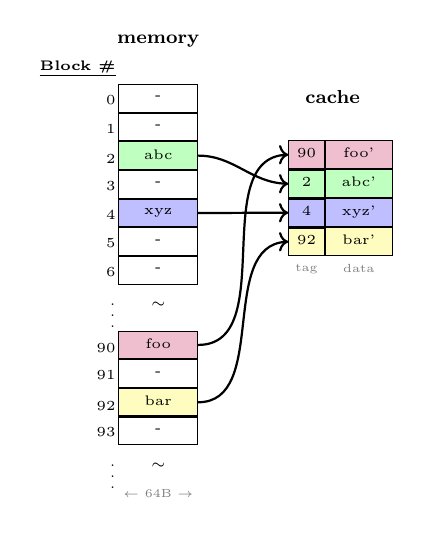
\begin{tikzpicture}[
  % Define colors
  lightblue/.style={draw, fill=blue!25},
  lightgreen/.style={draw, fill=green!25},
  lightyellow/.style={draw, fill=yellow!25},
  lightpurple/.style={draw, fill=purple!25},
  whiteblock/.style={draw, fill=white},
  % Base style for boxes
  basebox/.style={draw, minimum height=0.35cm, inner sep=1pt, font=\tiny, text depth=0.1em},
  % Styles inheriting from basebox
  membox/.style={basebox, minimum width=1.0cm},
  tagbox/.style={basebox, minimum width=0.45cm},
  databox/.style={basebox, minimum width=0.85cm},
  numcell/.style={font=\tiny, inner sep=1pt},
  scale=0.85, transform shape
]

  % Memory matrix
  \matrix[matrix of nodes,
          column sep=0pt, row sep=0pt,
          ampersand replacement=\&,
          column 1/.style={numcell, anchor=east},
          column 2/.style={membox},
          nodes in empty cells] (mem) {
    |[font=\tiny\bfseries]| \underline{Block \#} \& |[draw=none]| \\
    0 \& |[whiteblock]| - \\
    1 \& |[whiteblock]| - \\
    2 \& |[lightgreen]| abc \\
    3 \& |[whiteblock]| - \\
    4 \& |[lightblue]| xyz \\
    5 \& |[whiteblock]| - \\
    6 \& |[whiteblock]| - \\
    |[font=\tiny]| \vdots \& |[draw=none, font=\tiny]| $\sim$ \\
    90 \& |[lightpurple]| foo \\
    91 \& |[whiteblock]| - \\
    92 \& |[lightyellow]| bar \\
    93 \& |[whiteblock]| - \\
    |[font=\tiny]| \vdots \& |[draw=none, font=\tiny]| $\sim$ \\
  };

  % Memory title
  \node[anchor=south, font=\footnotesize\bfseries] at (mem-1-2.north) {memory};

  % 64B width indicator
  \node[anchor=north, font=\tiny, gray] at (mem-14-2.south) {$\leftarrow$ 64B $\rightarrow$};

  % Cache matrix with tag and data columns
  \matrix[matrix of nodes,
          column sep=0pt, row sep=0pt,
          ampersand replacement=\&,
          column 1/.style={tagbox},
          column 2/.style={databox},
          right=1.2cm of mem-5-2.east, anchor=west] (cache) {
    |[draw=none, font=\tiny]| \& |[draw=none]| \\
    |[lightpurple]| 90 \& |[lightpurple]| foo' \\
    |[lightgreen]| 2 \& |[lightgreen]| abc' \\
    |[lightblue]| 4 \& |[lightblue]| xyz' \\
    |[lightyellow]| 92 \& |[lightyellow]| bar' \\
  };

  % Cache title
  \node[anchor=south, font=\footnotesize\bfseries] at ($(cache-1-1.north)!0.5!(cache-1-2.north)$) {cache};

  % Tag/Data labels below cache
  \node[anchor=north, font=\tiny, gray] at (cache-5-1.south) {tag};
  \node[anchor=north, font=\tiny, gray] at (cache-5-2.south) {data};

  % Arrows from memory to cache
  \draw[->, thick] (mem-10-2.east) to[out=0, in=180] (cache-2-1.west);
  \draw[->, thick] (mem-4-2.east) to[out=0, in=180] (cache-3-1.west);
  \draw[->, thick] (mem-6-2.east) to[out=0, in=180] (cache-4-1.west);
  \draw[->, thick] (mem-12-2.east) to[out=0, in=180] (cache-5-1.west);

\end{tikzpicture}%
}

\usetheme{Madrid}
\setbeamertemplate{navigation symbols}{}

\title{Cache Memory}
\author{Computer Architecture 2360267}
\date{2025, Lecture \#3}

\begin{document}

\frame{\titlepage}

\begin{frame}{Outline}
\tableofcontents
\end{frame}

\section{Overview}

\begin{frame}{Processor--Memory Gap (summary)}
\begin{columns}[c]

\begin{column}{0.70\textwidth}
\centering
\includegraphics[width=\textwidth]{figures/processor_memory_gap.png}\\[0.1cm]
{\tiny Source: Efnusheva et al., IJCSIT 2017}
\end{column}
\begin{column}{0.28\textwidth}
\small
\begin{itemize}
  \item CPU improved $\sim$60\%/year
  \item DRAM improved $\sim$7\%/year
  \item Gap grew $\sim$50\%/year
  \item Motivation for caches
\end{itemize}
\end{column}
\end{columns}
\end{frame}

\begin{frame}{Memory Trade-Offs}
\begin{itemize}
  \item Large (dense) memories are \textbf{slow}
  \item Fast memories are \textbf{small}, expensive and consume high power
  \item Goal: give the processor the feeling that it has a memory which is large (dense), fast, consumes low power, and cheap
  \item Solution: a hierarchy of memories
\end{itemize}

\vspace{0.3cm}
\begin{center}
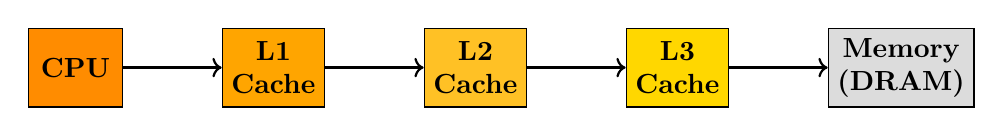
\begin{tikzpicture}[scale=0.8]
  % Define colors for the hierarchy
  \definecolor{cpucolor}{RGB}{255,140,0}      % Orange
  \definecolor{l1color}{RGB}{255,165,0}       % Orange
  \definecolor{l2color}{RGB}{255,193,37}      % Yellow-orange
  \definecolor{l3color}{RGB}{255,215,0}       % Gold
  \definecolor{memcolor}{RGB}{220,220,220}    % Light gray
  
  % Memory hierarchy boxes
  \node[rectangle, draw, fill=cpucolor, minimum width=1.2cm, minimum height=1cm, align=center, font=\bfseries] (cpu) at (0,0) {CPU};
  \node[rectangle, draw, fill=l1color, minimum width=1.2cm, minimum height=1cm, align=center, right=1.25cm of cpu, font=\bfseries] (l1) {L1\\Cache};
  \node[rectangle, draw, fill=l2color, minimum width=1.2cm, minimum height=1cm, align=center, right=1.25cm of l1, font=\bfseries] (l2) {L2\\Cache};
  \node[rectangle, draw, fill=l3color, minimum width=1.2cm, minimum height=1cm, align=center, right=1.25cm of l2, font=\bfseries] (l3) {L3\\Cache};
  \node[rectangle, draw, fill=memcolor, minimum width=1.2cm, minimum height=1cm, align=center, right=1.25cm of l3, font=\bfseries] (mem) {Memory\\(DRAM)};
  
  % Arrows between boxes
  \draw[->, thick] (cpu.east) -- (l1.west);
  \draw[->, thick] (l1.east) -- (l2.west);
  \draw[->, thick] (l2.east) -- (l3.west);
  \draw[->, thick] (l3.east) -- (mem.west);
\end{tikzpicture}
\end{center}
\begin{center}
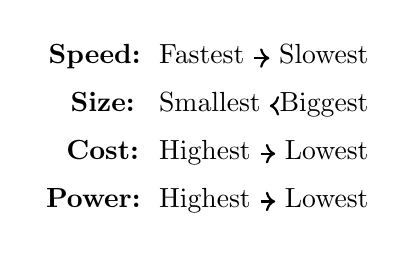
\begin{tikzpicture}
  \matrix[matrix of nodes,
    column sep=0pt,
    row sep=2pt,
    ampersand replacement=\&,
    nodes={anchor=center, text height=1.5ex, text depth=0.5ex},
    column 1/.style={nodes={font=\bfseries, anchor=east, minimum width=1.2cm}},
    column 2/.style={nodes={anchor=west}},
    column 3/.style={nodes={minimum width=5cm}},
    column 4/.style={nodes={anchor=east}},
  ] (m) {
    Speed: \& Fastest \& \& Slowest \\
    Size: \& Smallest \& \& Biggest \\
    Cost: \& Highest \& \& Lowest \\
    Power: \& Highest \& \& Lowest \\
  };
  % Draw arrows
  \foreach \row in {1,2,3,4} {
    \draw[->, thick] (m-\row-2.east) -- (m-\row-4.west);
  }
\end{tikzpicture}
\end{center}
\end{frame}

\begin{frame}{Why Hierarchy Works}
\begin{itemize}
  \item \textbf{Temporal Locality (Locality in Time):}
  \begin{itemize}
    \item If an item is referenced, it will tend to be referenced again soon
    \item Example: code and variables in loops
  \end{itemize}
  $\Rightarrow$ \textbf{Keep recently accessed data closer to the processor}
  
  \vspace{0.5cm}
  
  \item \textbf{Spatial Locality (Locality in Space):}
  \begin{itemize}
    \item If an item is referenced, nearby items tend to be referenced soon
    \item Example: scanning an array
  \end{itemize}
  $\Rightarrow$ \textbf{Move contiguous blocks closer to the processor}
  
  \vspace{0.5cm}
  
  \item \textbf{Locality + smaller HW is faster + Amdahl's law}\\
  $\Rightarrow$ \textbf{memory hierarchy}
\end{itemize}
\end{frame}

\begin{frame}{Memory Hierarchy: Terminology}
\begin{itemize}
  \item \textbf{For each memory level, define the following:}
  \begin{itemize}
    \item \textcolor{green!60!black}{\textbf{Hit:}} data at the requested address is available in the cache level
    \item \textcolor{green!60!black}{\textbf{Miss:}} data at the requested address is not available in the cache level
    \item \textcolor{green!60!black}{\textbf{Hit Rate:}} the fraction of accesses that hit in that cache level
    \begin{itemize}
      \item For L1 cache: $\frac{\text{\#L1 hits}}{\text{\#data accesses in the program}}$
      \item For L2 cache: $\frac{\text{\#L2 hits}}{\text{\#L1 misses}}$
    \end{itemize}
    \item \textcolor{green!60!black}{\textbf{Hit Time:}} time from data request until data received when hitting in the cache level; includes the time to determine hit/miss
    \item \textcolor{green!60!black}{\textbf{Miss Rate}} = $1 - (\text{Hit Rate})$
    \item \textcolor{green!60!black}{\textbf{Miss Penalty:}} Time to replace a block in the upper level + Time to deliver the block to the processor
  \end{itemize}

  \vspace{0.15cm}

  \item \textbf{Average memory-access time =}\\
  \hspace{1cm} $t_{\text{effective}} = (\text{Hit time} \times \text{Hit Rate}) + (\text{Miss Time} \times \text{Miss rate})$\\
  \hspace{2.2cm} $= (\text{Hit time} \times \text{Hit Rate}) + (\text{Miss Time} \times (1-\text{Hit rate}))$
  \begin{itemize}
    \item If hit rate is close to 1, $t_{\text{effective}}$ is close to hit time
  \end{itemize}
\end{itemize}
\end{frame}

\begin{frame}{Effective Memory Access Time}
\begin{itemize}
  \item \textbf{Cache -- holds a subset of the memory}
  \begin{itemize}
    \item Hopefully -- the subset being used now
  \end{itemize}
  
  \item \textbf{Effective memory access time}
  \begin{itemize}
    \item $t_{\text{effective}} = (t_{\text{cache}} \times \text{Hit Rate}) + (t_{\text{mem}} \times (1 - \text{Hit rate}))$
    \item $t_{\text{mem}}$ includes the time it takes to detect a cache miss
  \end{itemize}
  
  \item \textbf{Example}
  \begin{itemize}
    \item Assume $t_{\text{cache}} = 10$ nsec and $t_{\text{mem}} = 100$ nsec
  \end{itemize}
\end{itemize}

\begin{center}
\begin{tabular}{c|c|l}
\textbf{Hit Rate} & \textbf{$t_{\text{eff}}$ (nsec)} & \textbf{Computation} \\
\hline
0 & 100 & $(0.0 \times 10) + (1.0 \times 100)$ \\
50 & 55 & $(0.5 \times 10) + (0.5 \times 100)$ \\
90 & 19 & $(0.9 \times 10) + (0.1 \times 100)$ \\
99 & 10.9 & $(0.99 \times 10) + (0.01 \times 100)$ \\
99.9 & 10.1 & $(0.999 \times 10) + (0.001 \times 100)$ \\
\end{tabular}
\end{center}

\begin{itemize}
  \item $\frac{t_{\text{mem}}}{t_{\text{cache}}}$ ratio increases $\Rightarrow$ hit-rate is more important
\end{itemize}
\end{frame}

\section{Cache Organization}

\begin{frame}{Cache: Main Idea}
\begin{columns}[T]
\begin{column}{0.65\textwidth}
\begin{itemize}
  \item \textcolor{blue}{\textbf{The cache holds a small part of the memory}}
  \begin{itemize}
    \item Need to map parts of memory into the cache
  \end{itemize}
  
  \item \textcolor{blue}{\textbf{Memory is (logically) partitioned into blocks}}
  \begin{itemize}
    \item Typical block size is 32 or 64 bytes
    \item Blocks are aligned
  \end{itemize}
  
  \item \textcolor{blue}{\textbf{The cache is partitioned into cache lines}}
  \begin{itemize}
    \item Each cache line holds a memory block
    \item Only a subset of the memory blocks are mapped to the cache at a given time
    \item The cache views an address as:
  \end{itemize}
\end{itemize}

% Address format at the bottom of text
\begin{center}
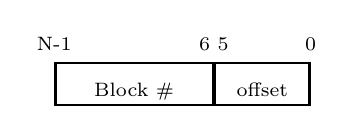
\begin{tikzpicture}[
    scale=1,
    box/.style={font=\scriptsize, minimum height=0.5cm, draw, thick, align=center, inner sep=2pt, text depth=0.1em, text height=1em}
]

  % Bottom row (actual fields, in boxes)
  \node[box, minimum width=2.0cm] (block) {Block \#};
  \node[box, minimum width=1.2cm, right=0cm of block] (offset) {offset};

  % Numbers above (plain text only, no boxes)
  \node[font=\scriptsize, above=0.03cm of block.north west, anchor=south] {N-1};
  \node[font=\scriptsize, above=0.03cm of block.north east, anchor=south] {6 5};
  \node[font=\scriptsize, above=0.03cm of offset.north east, anchor=south] {0};

\end{tikzpicture}
\end{center}
\end{column}

\begin{column}{0.35\textwidth}
\centering
\memoryCacheIllustration
\end{column}
\end{columns}
\end{frame}

\begin{frame}{Cache Lookup}
\begin{columns}[T]
\begin{column}{0.6\textwidth}
\begin{itemize}
  \item \textbf{Cache hit}
  \begin{itemize}
    \item Block is in the cache ---
    return data according to offset
  \end{itemize}

  \vspace{0.4cm}

  \item \textbf{Cache miss}
  \begin{itemize}
    \item Block is not in the cache
    \item Perform a cache line fill:
    \begin{itemize}
      \item Fetch block into fill buffer
      \item May require several bus cycles
      \item Write fill buffer into cache
    \end{itemize}
    \item May need to evict another block
    \begin{itemize}
      \item Make room for the new block
    \end{itemize}
  \end{itemize}
\end{itemize}
\end{column}

\begin{column}{0.4\textwidth}
\memoryCacheIllustration
\end{column}
\end{columns}
\end{frame}

\begin{frame}{Fully Associative (FA) Cache}
\begin{columns}[T]
\begin{column}{0.42\textwidth}
\small
\begin{itemize}
  \item Any block can map to any line
  \item All tags compared in parallel
  \item On match, return data at offset
\end{itemize}
\vspace{0.3cm}
\textcolor{green!70!black}{\textbf{+}} Lowest conflict misses\\
\textcolor{red!70!black}{\textbf{--}} Many comparators (area/power)
\end{column}
\begin{column}{0.58\textwidth}
\centering
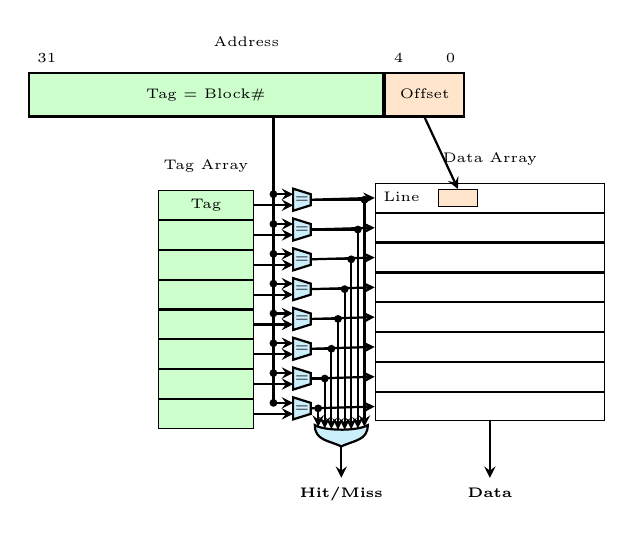
\begin{tikzpicture}[
    % Address field styles
    addrfield/.style={draw, thick, minimum height=0.55cm, font=\tiny, text depth=0.1em},
    tagfield/.style={addrfield, fill=green!20, minimum width=4.5cm},
    offsetfield/.style={addrfield, fill=orange!20, minimum width=1cm},
    % Cell styles for matrix
    basecell/.style={draw, minimum height=0.2cm, font=\tiny, inner sep=3pt},
    tagcell/.style={basecell, minimum width=1.2cm, fill=green!20},
    datacell/.style={basecell, minimum width=2.8cm, fill=white, text width=2.7cm, align=left},
    offsetbox/.style={basecell, minimum width=0.5cm, fill=orange!20},
    label/.style={font=\tiny},
    data_connector/.style={circle, fill, inner sep=1pt},
    scale=1, transform shape
]

% Address breakdown at top
\node[tagfield] (tag_field) {Tag = Block\#};
\node[offsetfield, anchor=west] (offset_field) at (tag_field.east) {Offset};
\node[label, anchor=south west] at (tag_field.north west) {31};
\node[label, anchor=south west] at (offset_field.north west) {4};
\node[label, anchor=south east] (zero) at (offset_field.north east) {0};
\node[label, anchor=south] (addr_title) at ([yshift=2mm]$(tag_field.north west)!0.5!(offset_field.north east)$) {Address};

% Tag matrix
\matrix[matrix of nodes,
        column sep=0pt, row sep=0pt,
        ampersand replacement=\&,
        anchor=north] at ([yshift=-8mm]tag_field.south) (tag) {
  |[tagcell]| Tag \\
  |[tagcell]| \phantom{Tag} \\
  |[tagcell]| \phantom{Tag} \\
  |[tagcell]| \phantom{Tag} \\
  |[tagcell]| \phantom{Tag} \\
  |[tagcell]| \phantom{Tag} \\
  |[tagcell]| \phantom{Tag} \\
  |[tagcell]| \phantom{Tag} \\
};
\node[label, above=1mm of tag-1-1.north] {Tag Array};

% Comparators for each row
\foreach \i in {1,...,8} {
    \node[muxdemux, muxdemux def={Lh=0.5, Rh=0.25, NL=2, NB=1, w=0.4},
          external pins width=0, fill=cyan!20, anchor=lpin 2] (comp\i) at ([xshift=0.5cm]tag-\i-1.east) {};
    \node[font=\fontsize{3}{3}\selectfont] at (comp\i.center) {=};
}

% Data matrix
\matrix[matrix of nodes,
        column sep=0pt, row sep=0pt, inner sep=3pt,
        ampersand replacement=\&,
        anchor=north west] (data) at ([xshift=0.7cm,yshift=3.25mm]comp1.rpin 1) {
  |[datacell]| Line\phantom{Tag} \\
  |[datacell]| \phantom{Tag} \\
  |[datacell]| \phantom{Tag} \\
  |[datacell]| \phantom{Tag} \\
  |[datacell]| \phantom{Tag} \\
  |[datacell]| \phantom{Tag} \\
  |[datacell]| \phantom{Tag} \\
  |[datacell]| \phantom{Tag} \\
};
\node[label, above=1mm of data-1-1.north] {Data Array};

% Orange offset box on first data line
\node[offsetbox, anchor=west] at ([xshift=0.8cm]data-1-1.west) (thedata) {};

% Connect tag input to all comparators
\foreach \i in {1,...,8} {
    \draw[->, >=stealth, thick] ([xshift=2.5mm]tag_field.south -| tag-1-1.east) -- ([xshift=2.5mm]tag-\i-1.east |- comp\i.lpin 1) node[data_connector] {} -- (comp\i.lpin 1);
}

% Connect offset to data
\draw[->, >=stealth, thick] (offset_field.south) -- (thedata.north);

% Connect tag array to comparators, comparators to data array
\foreach \i in {1,...,8} {
    \draw[->, >=stealth, thick] (tag-\i-1.east) -- (comp\i.lpin 2);
    \draw[->, >=stealth, thick] (comp\i.rpin 1) -- (data-\i-1.west);
}

% OR gate for hit/miss
\node[or port, number inputs=8, anchor=north, external pins width=0, fill=cyan!20,
      xscale=0.6, yscale=0.25, rotate=-90, below right=0.4cm and 0.5cm of comp8.south, anchor=out] (or_gate) {};

% Connect comparators to OR gate
\foreach \i in {1,...,8} {
    \draw[->, >=stealth, thick] (comp\i.rpin 1) -- (comp\i.rpin 1 -| or_gate.bin \i) node[data_connector] {} -- (or_gate.bin \i);
}

% Hit/Miss output
\node[label, below=0.4cm of or_gate.bout, font=\tiny\bfseries] (hit_miss) {Hit/Miss};
\draw[->, >=stealth, thick] (or_gate.bout) -- (hit_miss.north);

% Data output
\node[label, font=\tiny\bfseries, anchor=north] (data_out) at (data-8-1.south |- hit_miss.north east) {Data};
\draw[->, >=stealth, thick] (data-8-1.south) -- (data_out.north);

\end{tikzpicture}
\end{column}
\end{columns}
\end{frame}

\begin{frame}{Valid Bit}

\begin{columns}
\begin{column}{0.4\textwidth}
\centering
\begin{itemize}
  \item Cache starts empty; each line needs a \textbf{valid} bit.
  \item Valid set on fill; lines may be invalidated later.
\end{itemize}

\end{column}
\begin{column}{0.5\textwidth}
\centering
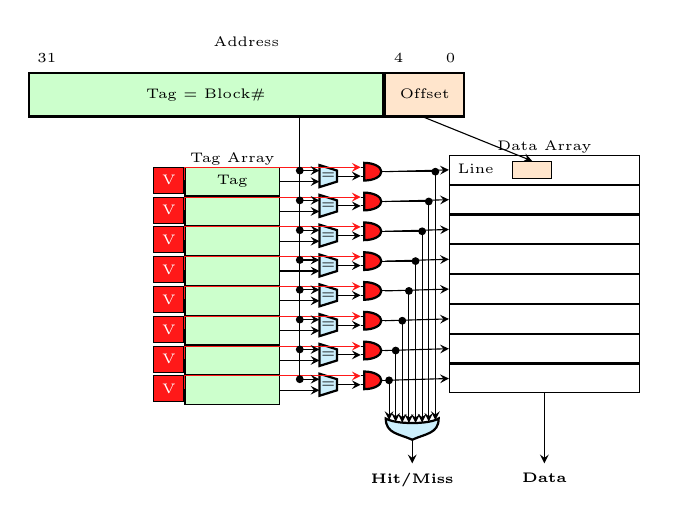
\begin{tikzpicture}[
    % Address field styles
    addrfield/.style={draw, thick, minimum height=0.55cm, font=\tiny, text depth=0.1em},
    tagfield/.style={addrfield, fill=green!20, minimum width=4.5cm},
    offsetfield/.style={addrfield, fill=orange!20, minimum width=1cm},
    % Cell styles for matrix
    basecell/.style={draw, minimum height=0.2cm, font=\tiny, inner sep=3pt},
    validcell/.style={basecell, minimum width=0.3cm, fill=red!90, text=white},
    tagcell/.style={basecell, minimum width=1.2cm, fill=green!20},
    datacell/.style={basecell, minimum width=2.3cm, fill=white, text width=2.2cm, align=left},
    offsetbox/.style={basecell, minimum width=0.5cm, fill=orange!20},
    label/.style={font=\tiny},
    data_connector/.style={circle, fill, inner sep=1pt},
    scale=1, transform shape
]

% Address breakdown at top
\node[tagfield] (tag_field) {Tag = Block\#};
\node[offsetfield, anchor=west] (offset_field) at (tag_field.east) {Offset};
\node[label, anchor=south west] at (tag_field.north west) {31};
\node[label, anchor=south west] at (offset_field.north west) {4};
\node[label, anchor=south east] (zero) at (offset_field.north east) {0};
\node[label, anchor=south] (addr_title) at ([yshift=2mm]$(tag_field.north west)!0.5!(offset_field.north east)$) {Address};

% Valid+Tag matrix - use explicit style on each cell
\matrix[matrix of nodes,
        column sep=0pt, row sep=0pt,
        ampersand replacement=\&,
        anchor=north] at ([xshift=24mm,yshift=-5mm]tag_field.south west) (vtag) {
  |[validcell]| V \& |[tagcell]| Tag \\
  |[validcell]| V \& |[tagcell]| \phantom{Tag} \\
  |[validcell]| V \& |[tagcell]| \phantom{Tag} \\
  |[validcell]| V \& |[tagcell]| \phantom{Tag} \\
  |[validcell]| V \& |[tagcell]| \phantom{Tag} \\
  |[validcell]| V \& |[tagcell]| \phantom{Tag} \\
  |[validcell]| V \& |[tagcell]| \phantom{Tag} \\
  |[validcell]| V \& |[tagcell]| \phantom{Tag} \\
};



% Comparators and AND gates for each row
\foreach \i in {1,...,8} {
    % Comparator
    \node[muxdemux, muxdemux def={Lh=0.5, Rh=0.25, NL=2, NB=1, w=0.4},
          external pins width=0, fill=cyan!20, anchor=lpin 2] (comp\i) at ([xshift=0.5cm]vtag-\i-2.east) {};
    \node[font=\fontsize{3}{3}\selectfont] at (comp\i.center) {=};

    % AND gate
    \node[and port, number inputs=2, anchor=in 2, external pins width=0, fill=red!90,
      xscale=0.2, yscale=0.2] (and_gate_\i) at ([xshift=3mm]comp\i.rpin 1) {};
}




% Data matrix - positioned to align vertically with vtag (same y as vtag-1-2)
\matrix[matrix of nodes,
        column sep=0pt, row sep=0pt, inner sep=3pt,
        ampersand replacement=\&,
        anchor=north west] (data) at ([xshift=0.7cm,yshift=3.25mm]and_gate_1.out) {
  |[datacell]| Line\phantom{Tag} \\
  |[datacell]| \phantom{Tag} \\
  |[datacell]| \phantom{Tag} \\
  |[datacell]| \phantom{Tag} \\
  |[datacell]| \phantom{Tag} \\
  |[datacell]| \phantom{Tag} \\
  |[datacell]| \phantom{Tag} \\
  |[datacell]| \phantom{Tag} \\
};

% Orange offset box on first data line
\node[offsetbox, anchor=west] at ([xshift=8mm]data-1-1.west) (thedata) {};

% Labels
\node[label, above=-1mm of vtag-1-2.north] {Tag Array};
\node[label, above=-1mm of data-1-1.north] {Data Array};

% OR gate for hit/miss
\node[or port, number inputs=8, anchor=north, external pins width=0, fill=cyan!20,
      xscale=0.6, yscale=0.25, rotate=-90, below right=0.7cm and 0.5cm of and_gate_8.south, anchor=out] (or_gate) {};


\foreach \i in {1,...,8} {
    % Connections
    \draw[->, >=stealth] (vtag-\i-2.east) -- (comp\i.lpin 2);
    \draw[->, >=stealth] (comp\i.rpin 1) -- (and_gate_\i.in 2);
    \draw[->, >=stealth] (and_gate_\i.out) -- (data-\i-1.west);
    \draw[->, >=stealth, color=red!90] (vtag-\i-1.east) |- (and_gate_\i.in 1);
}

% Connect tag input to all comparators
\foreach \i in {1,...,8} {
    \draw[->, >=stealth] ([xshift=2.5mm]tag_field.south -| vtag-1-2.east) -- ([xshift=2.5mm]vtag-\i-2.east |- comp\i.lpin 1) node[data_connector] {} -- (comp\i.lpin 1);
}

\draw[->, >=stealth] (offset_field.south) -- (thedata.north);


% Connect AND gates to OR gate
\foreach \i in {1,...,8} {
    \draw[->, >=stealth] (and_gate_\i.out) -- (and_gate_\i.out -| or_gate.bin \i) node[data_connector] {} -- (or_gate.bin \i);
}

% Hit/Miss output
\node[label, below=0.3cm of or_gate.bout, font=\tiny\bfseries] (hit_miss) {Hit/Miss};
\draw[->, >=stealth] (or_gate.bout) -- (hit_miss.north);

% Data output
\node[label, font=\tiny\bfseries, anchor=north] (data_out) at (data-8-1.south |- hit_miss.north east) {Data};
\draw[->, >=stealth] (data-8-1.south) -- (data_out.north);

\end{tikzpicture}
\end{column}
\end{columns}
\end{frame}

\begin{frame}{Direct-Mapped (DM) Cache}
\begin{columns}[T]
\begin{column}{0.38\textwidth}
\begin{itemize}
  \item Each memory block maps to exactly \textbf{one} cache line
  \item Block number split into \textbf{set} + \textbf{tag}
  \item Set: lower $n$ bits $\rightarrow$ selects one of $2^n$ lines
  \item Tag: upper bits $\rightarrow$ compared with stored tag
  \item Single comparator needed
\end{itemize}
\end{column}
\begin{column}{0.60\textwidth}
\centering
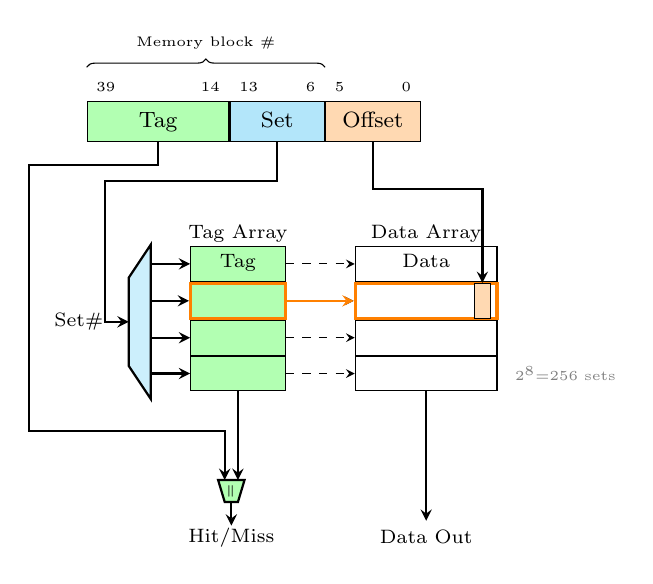
\begin{tikzpicture}[scale=1, transform shape,
    % Address box styles
    addrbox/.style={rectangle, draw, minimum height=0.5cm, font=\footnotesize, text depth=0.1em},
    tagbox/.style={addrbox, fill=green!30, minimum width=1.8cm},
    setbox/.style={addrbox, fill=cyan!30, minimum width=1.2cm},
    offsetbox/.style={addrbox, fill=orange!30, minimum width=1.2cm},
    % Cell styles for matrices
    cellstyle/.style={rectangle, draw, minimum width=1.2cm, minimum height=0.3cm,
                     text depth=0.1cm, text height=0.2cm, font=\tiny, inner sep=2pt},
    tagcell/.style={cellstyle, fill=green!30},
    datacell/.style={cellstyle, minimum width=1.8cm},
    offsetcell/.style={cellstyle, fill=orange!30, minimum width=2mm},
    decoder/.style={muxdemux, muxdemux def={Lh=2, Rh=3.5, NB=0, NL=1, NR=4, w=0.5, square pins=0},
                   external pins width=0, fill=cyan!20},
    arrow/.style={->, >=stealth, thick},
    dasharrow/.style={dashed, ->, >=stealth},
    junction/.style={circle, fill=black, inner sep=0pt, minimum size=3pt}
]

% Address bits at top
\node[tagbox] at (0,0) (tag) {Tag};
\node[setbox, right=0pt of tag] (set) {Set};
\node[offsetbox, right=0pt of set] (offset) {Offset};

% Bit labels - adjacent to boxes
\node[anchor=south west, font=\tiny] at (tag.north west) (block_end) {39};
\node[anchor=south east, font=\tiny] at (tag.north east) {14};
\node[anchor=south west, font=\tiny] at (set.north west) {13};
\node[anchor=south east, font=\tiny] at (set.north east) (block_start) {6};
\node[anchor=south west, font=\tiny] at (offset.north west) {5};
\node[anchor=south east, font=\tiny] at (offset.north east) {0};

% Brace above Tag+Set for "Memory block number"
\draw[decorate, decoration={brace, amplitude=3pt, raise=2pt}]
    (block_end.north west) -- (block_start.north east)
    node[midway, above=5pt, font=\tiny] {Memory block \#};

% Tag matrix
\matrix[matrix of nodes,
        column sep=0pt, row sep=0pt,
        ampersand replacement=\&,
        anchor=north] at ([xshift=-0.5cm, yshift=-1.2cm]set.south) (tagmat) {
  |[tagcell]| {\scriptsize Tag} \\
  |[tagcell, very thick, draw=orange]| \phantom{Tag} \\
  |[tagcell]| \phantom{Tag} \\
  |[tagcell]| \phantom{Tag} \\
};

% Data matrix - same y as tag
\matrix[matrix of nodes,
        column sep=0pt, row sep=0pt,
        ampersand replacement=\&,
        anchor=north west] at ([xshift=0.6cm]tagmat.north east) (datamat) {
  |[datacell]| {\scriptsize Data} \\
  |[datacell, very thick, draw=orange]| \phantom{Data} \\
  |[datacell]| \phantom{Data} \\
  |[datacell]| \phantom{Data} \\
};
\node[offsetcell, anchor=east] at ([xshift=-1mm]datamat-2-1.east) (thedata) {};

% Decoder
\node[decoder, anchor=rpin 1] at ([xshift=-0.5cm]tagmat-1-1.west) (decoder) {};

% Comparator
\node[muxdemux, muxdemux def={Lh=0.6, Rh=0.3, NL=2, NB=1, w=0.5},
      external pins width=0, fill=green!30, rotate=270, anchor=lpin 1] at ([yshift=-1cm]tagmat.south) (comp) {};
\node[font=\fontsize{4}{4}\selectfont, rotate=90] at (comp.center) {=};

% Labels
\node[left=2mm of decoder.lpin 1, font=\scriptsize] (setlabel) {Set\#};
\node[above=-2mm of tagmat.north, anchor=south, font=\scriptsize] {Tag Array};
\node[above=-2mm of datamat.north, anchor=south, font=\scriptsize] {Data Array};
\node[below=2mm of comp.rpin 1, font=\scriptsize] (hitmiss) {Hit/Miss};
\node[font=\scriptsize] at (hitmiss -| datamat) (dataout) {Data Out};
\node[right=1mm of datamat-4-1.east, font=\tiny, text=gray] {$2^8$=256 sets};

% Connections
% Set to decoder
\draw[arrow] (set.south) -- ++(0,-0.5) -| ([xshift=-3mm]decoder.lpin 1) -- (decoder.lpin 1);

% Tag to comparator
\draw[arrow] (tag.south) -- ++(0,-3mm) -| ([xshift=-2mm, yshift=-5mm]setlabel.west |- tagmat-4-1.south) -| (comp.lpin 2);

% Offset to data
\draw[arrow] (offset.south) -- ++(0,-0.6) -| (thedata.north);

% Decoder to tag array
\foreach \i in {1,...,4} {
    \draw[arrow] (decoder.rpin 1 |- tagmat-\i-1.west) -- (tagmat-\i-1.west);
}

% Tag to data (dashed)
\foreach \i in {1,...,4} {
    \draw[dasharrow] (tagmat-\i-1.east) -- (datamat-\i-1.west);
}

% Selected line highlight (row 2)
\draw[arrow, thick, orange] (tagmat-2-1.east) -- (datamat-2-1.west);

% Tag array to comparator (from south of matrix)
\draw[arrow] (tagmat-4-1.south) -- (comp.lpin 1);

% Comparator output
\draw[arrow] (comp.rpin 1) -- ++(0,-0.3);

% Data out (from bottom of matrix)
\draw[arrow] (datamat-4-1.south) -- (dataout.north);

\end{tikzpicture}
\end{column}
\end{columns}
\end{frame}

\begin{frame}{Direct-Mapped Cache -- Properties}
\begin{columns}[T]
\begin{column}{0.48\textwidth}
\textbf{Cache Size Calculation:}
\begin{itemize}
  \item Cache size = \#sets $\times$ block size
  \item Example: $2^8 \times 2^6 = 2^{14}$ bytes = 16KB
\end{itemize}
\vspace{0.3cm}
\textbf{Conflict Behavior:}
\begin{itemize}
  \item Two blocks with same set bits $\rightarrow$ map to same line
  \item Only one can reside at a time
  \item Min distance between conflicts = cache size
\end{itemize}
\end{column}
\begin{column}{0.48\textwidth}
\textbf{Advantages:}
\begin{itemize}
  \item Low power and area
  \item Simple replacement -- only one possible victim
  \item Fast lookup -- single comparator
\end{itemize}
\vspace{0.3cm}
\textbf{Disadvantages:}
\begin{itemize}
  \item Lower hit rate than Fully Associative
  \item \textbf{Conflict misses}: victim needed even when cache not full
  \item (FA cache has only capacity misses)
\end{itemize}
\end{column}
\end{columns}
\end{frame}

\begin{frame}{Direct-Mapped Cache -- Example}
\begin{columns}[T]
\begin{column}{0.45\textwidth}
\textbf{Given:}
\begin{itemize}
  \item Line size: 32 bytes $\rightarrow$ 5 offset bits
  \item Cache size: 16KB = $2^{14}$ bytes
  \item \#lines = $\frac{2^{14}}{2^5} = 2^9 = 512$
  \item \#sets = \#lines = 512
  \item \#set bits = 9 bits
  \item \#tag bits = $32 - (9+5) = 18$ bits
\end{itemize}
\end{column}
\begin{column}{0.52\textwidth}
\textbf{Lookup Address:} \texttt{0x12345678}\\[0.2cm]
\texttt{\small 0001 0010 0011 0100 0101 0110 0111 1000}\\[0.3cm]
\centering
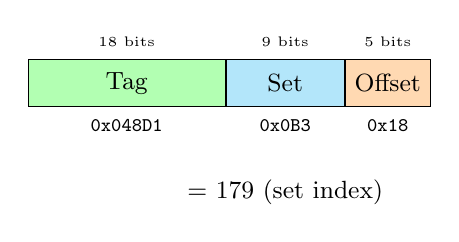
\begin{tikzpicture}[scale=0.9,
    tagbox/.style={rectangle, draw, fill=green!30, minimum height=0.6cm, font=\small},
    setbox/.style={rectangle, draw, fill=cyan!30, minimum height=0.6cm, font=\small},
    offsetbox/.style={rectangle, draw, fill=orange!30, minimum height=0.6cm, font=\small}
]
\node[tagbox, minimum width=2.5cm] at (0,0) (tag) {Tag};
\node[setbox, minimum width=1.5cm, right=0pt of tag] (set) {Set};
\node[offsetbox, minimum width=1cm, right=0pt of set] (offset) {Offset};

\node[above=1pt of tag.north, font=\tiny] {18 bits};
\node[above=1pt of set.north, font=\tiny] {9 bits};
\node[above=1pt of offset.north, font=\tiny] {5 bits};

\node[below=1pt of tag.south, font=\scriptsize] {\texttt{0x048D1}};
\node[below=1pt of set.south, font=\scriptsize] {\texttt{0x0B3}};
\node[below=1pt of offset.south, font=\scriptsize] {\texttt{0x18}};

\node[below=0.8cm of set.south, font=\small] {= 179 (set index)};
\end{tikzpicture}
\end{column}
\end{columns}
\end{frame}

\begin{frame}[fragile]{2-Way Set Associative (2W SA)}
\begin{center}
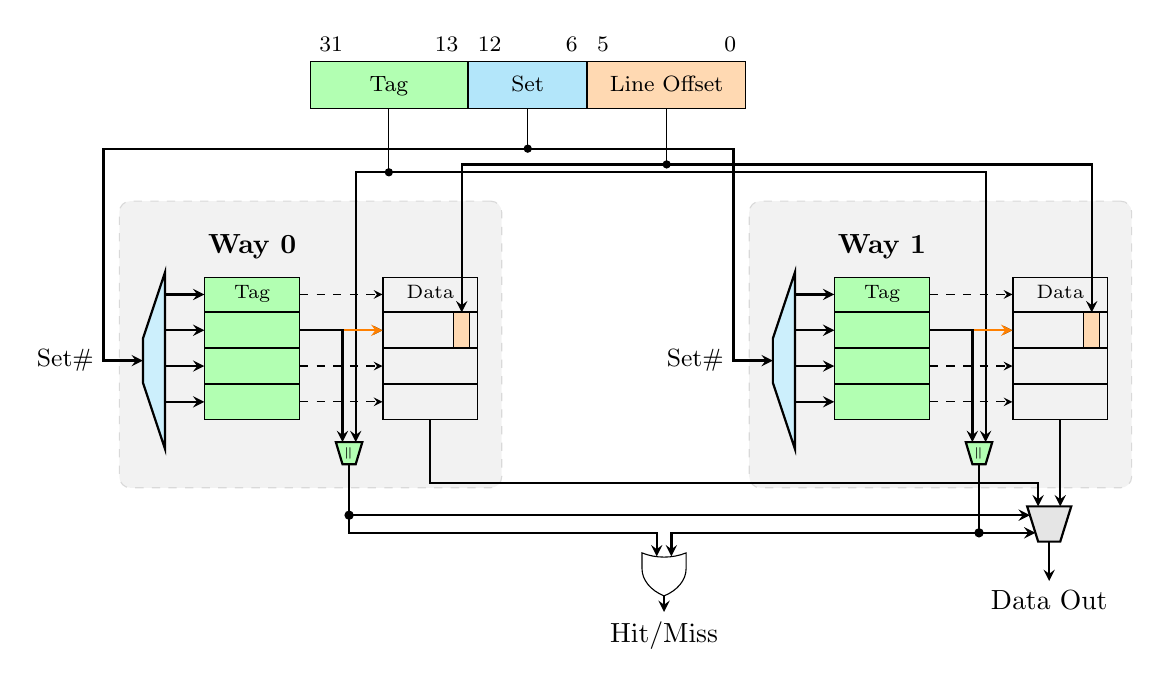
\begin{tikzpicture}[scale=1, transform shape,
    % Style definitions
    addrbox/.style={rectangle, draw, minimum height=0.6cm, font=\footnotesize, text depth=0.1em},
    tagbox/.style={addrbox, fill=green!30, minimum width=2cm},
    setbox/.style={addrbox, fill=cyan!30, minimum width=1.5cm},
    offsetbox/.style={addrbox, fill=orange!30, minimum width=2cm},
    cellstyle/.style={rectangle, draw, minimum width=1.2cm, minimum height=0.3cm,
                     text depth=0.1cm, text height=0.2cm, font=\tiny, inner sep=2pt},
    tagcell/.style={cellstyle, fill=green!30},
    datacell/.style={cellstyle},
    offsetcell/.style={cellstyle, fill=orange!30, minimum width=2mm},
    decoder/.style={muxdemux, muxdemux def={Lh=1, Rh=4, NB=0, NL=1, NR=4, w=0.5, square pins=0},
                   external pins width=0, fill=cyan!20},
    arrow/.style={->, >=stealth, thick},
    dasharrow/.style={dashed, ->, >=stealth},
    orgatestyle/.style={or gate US, draw, logic gate inputs=nn, anchor=center,
                       minimum width=1cm, minimum height=0.8cm, rotate=90},
    junction/.style={circle, fill=black, inner sep=0pt, minimum size=3pt},
    data_connector/.style={circle, fill, inner sep=1.2pt}
]

% Address bits at top - shifted to the right
\node[tagbox] at (2,0) (tag) {Tag};
\node[setbox, right=0pt of tag] (set) {Set};
\node[offsetbox, right=0pt of set] (offset) {Line Offset};

% Bit labels - adjacent to boxes
\node[anchor=south west] at (tag.north west) {\footnotesize 31};
\node[anchor=south east] at (tag.north east) {\footnotesize 13};
\node[anchor=south west] at (set.north west) {\footnotesize 12};
\node[anchor=south east] at (set.north east) {\footnotesize 6};
\node[anchor=south west] at (offset.north west) {\footnotesize 5};
\node[anchor=south east] at (offset.north east) {\footnotesize 0};

% Way 0 Tag matrix
\matrix[matrix of nodes,
        column sep=0pt, row sep=0pt,
        ampersand replacement=\&,
        anchor=north] at ([xshift=-3.5cm, yshift=-2cm]set.south) (tag0) {
  |[tagcell]| {\scriptsize Tag} \\
  |[tagcell]| \phantom{Tag} \\
  |[tagcell]| \phantom{Tag} \\
  |[tagcell]| \phantom{Tag} \\
};

% Way 0 decoder (demux)
\node[decoder, anchor=rpin 1] at ([xshift=-0.5cm]tag0-1-1.west) (decoder0) {};
\node[font=\small, anchor=east] at ([xshift=-5mm]decoder0.lpin 1) {Set\#};

% Way 0 Data matrix - same y as tag0
\matrix[matrix of nodes,
        column sep=0pt, row sep=0pt,
        ampersand replacement=\&,
        anchor=north west] at ([xshift=0.8cm]tag0.north east) (data0) {
  |[datacell]| {\scriptsize Data} \\
  |[datacell]| \phantom{Data} \\
  |[datacell]| \phantom{Data} \\
  |[datacell]| \phantom{Data} \\
};
% Orange box for line offset on second data line
\node[offsetcell, anchor=east] at ([xshift=-1mm]data0-2-1.east) (thedata0) {};

% Way 0 comparator
\node[muxdemux, muxdemux def={Lh=0.6, Rh=0.3, NL=2, NB=1, w=0.5},
      external pins width=0, fill=green!30, rotate=270] at ([xshift=5mm, yshift=-3mm]tag0.south east) (comp0) {};
\node[font=\fontsize{4}{4}\selectfont, rotate=90] at (comp0.center) {=};

% Way 0 label
\node[above=1mm of tag0-1-1.north] (way0label) {\textbf{Way 0}};

% Way 1 Tag matrix
\matrix[matrix of nodes,
        column sep=0pt, row sep=0pt,
        ampersand replacement=\&,
        anchor=north] at ([xshift=4.5cm, yshift=-2cm]set.south) (tag1) {
  |[tagcell]| {\scriptsize Tag} \\
  |[tagcell]| \phantom{Tag} \\
  |[tagcell]| \phantom{Tag} \\
  |[tagcell]| \phantom{Tag} \\
};

% Way 1 decoder (demux)
\node[decoder, anchor=rpin 1] at ([xshift=-0.5cm]tag1-1-1.west) (decoder1) {};
\node[font=\small, anchor=east] at ([xshift=-5mm]decoder1.lpin 1) {Set\#};

% Way 1 Data matrix - same y as tag1
\matrix[matrix of nodes,
        column sep=0pt, row sep=0pt,
        ampersand replacement=\&,
        anchor=north west] at ([xshift=0.8cm]tag1.north east) (data1) {
  |[datacell]| {\scriptsize Data} \\
  |[datacell]| \phantom{Data} \\
  |[datacell]| \phantom{Data} \\
  |[datacell]| \phantom{Data} \\
};
\node[offsetcell, anchor=east] at ([xshift=-1mm]data1-2-1.east) (thedata1) {};

% Way 1 comparator
\node[muxdemux, muxdemux def={Lh=0.6, Rh=0.3, NL=2, NB=1, w=0.5},
      external pins width=0, fill=green!30, rotate=270] at ([xshift=5mm, yshift=-3mm]tag1.south east) (comp1) {};
\node[font=\fontsize{4}{4}\selectfont, rotate=90] at (comp1.center) {=};

% Way 1 label
\node[above=1mm of tag1-1-1.north] (way1label) {\textbf{Way 1}};

% Background for ways
\begin{pgfonlayer}{background}
    \node[fit=(way0label)(decoder0)(tag0-1-1)(tag0-4-1)(data0-1-1)(data0-4-1)(comp0),
          fill=gray!10, draw=gray!30, dashed, rounded corners,
          inner sep=3mm] (way0bg) {};
    \node[fit=(way1label)(decoder1)(tag1-1-1)(tag1-4-1)(data1-1-1)(data1-4-1)(comp1),
          fill=gray!10, draw=gray!30, dashed, rounded corners,
          inner sep=3mm] (way1bg) {};
\end{pgfonlayer}

% OR gate - positioned between comparators
\node[orgatestyle, rotate=180, yscale=0.7, xscale=0.5] at ($(comp0)!0.5!(comp1) + (0,-1.5)$) (orgate) {};

% MUX - using muxdemux, rotated 270 degrees, positioned relative to data arrays
\node[muxdemux, muxdemux def={Lh=1, Rh=0.5, NL=2, NB=2, NR=1, w=0.8},
      external pins width=0, fill=gray!20, rotate=270,anchor=lpin 1] at ([yshift=-1.1cm]data1-4-1.south) (mux) {};

% Output labels
\node[below=2mm of orgate.east] (hitmiss) {Hit/Miss};
\node[below=0.5cm of mux.rpin 1] (dataout) {Data Out};

% Arrows from address bits to decoders with junction - initial line has no arrow
\draw (set.south) -- ++(0,-0.5) coordinate (setjunction);
\node[junction] at (setjunction) {};
\draw[arrow] (setjunction) -| ([xshift=-5mm]decoder0.lpin 1) -- (decoder0.lpin 1);
\draw[arrow] (setjunction) -| ([xshift=-5mm]decoder1.lpin 1) -- (decoder1.lpin 1);

% Arrows from address tag to comparators with junction - initial line has no arrow
\draw (tag.south) -- ++(0,-0.8) coordinate (tagjunction);
\node[junction] at (tagjunction) {};
\draw[arrow] (tagjunction) -| (comp0.lpin 1);
\draw[arrow] (tagjunction) -| (comp1.lpin 1);

% Arrows from offset to data arrays with junction - initial line has no arrow
\draw (offset.south) -- ++(0,-0.7) coordinate (offsetjunction);
\node[junction] at (offsetjunction) {};
\draw[arrow] (offsetjunction) -| (thedata0.north);
\draw[arrow] (offsetjunction) -| (thedata1.north);

% Decoder to tag arrays - straight horizontal lines
\foreach \i in {1,...,4} {
    \draw[arrow] (decoder0.rpin 1 |- tag0-\i-1.west) -- (tag0-\i-1.west);
    \draw[arrow] (decoder1.rpin 1 |- tag1-\i-1.west) -- (tag1-\i-1.west);
}

% Dashed lines from tag arrays to data arrays (each row)
\foreach \i in {1,...,4} {
    \draw[dasharrow] (tag0-\i-1.east) -- (data0-\i-1.west);
    \draw[dasharrow] (tag1-\i-1.east) -- (data1-\i-1.west);
}

% Selected line highlighting (example: line 2)
\draw[arrow, thick, orange] (tag0-2-1.east) -- (data0-2-1.west);
\draw[arrow, thick, orange] (tag1-2-1.east) -- (data1-2-1.west);

% Tag array output to comparator
\draw[arrow] (tag0-2-1.east) -| (comp0.lpin 2);
\draw[arrow] (tag1-2-1.east) -| (comp1.lpin 2);

% Data array to MUX connections
\draw[arrow] (data0-4-1.south) |- ([yshift=3mm]mux.lpin 2) -- (mux.lpin 2);
\draw[arrow] (data1-4-1.south) -- (mux.lpin 1);

% Comparator outputs to OR gate
\draw[arrow] (comp0.rpin 1) |- ([yshift=3mm]orgate.input 2) -- (orgate.input 2);
\draw[arrow] (comp1.rpin 1) |- ([yshift=3mm]orgate.input 1) -- (orgate.input 1);

% OR gate to Hit/Miss
\draw[arrow] (orgate.output) -- (hitmiss.north);

% Comparator to MUX select (using comp1 output)
\draw[arrow] (comp0.rpin 1 |- mux.bpin 1) node[data_connector] {} -- (mux.bpin 1);
\draw[arrow] (comp1.rpin 1 |- mux.bpin 2) node[data_connector] {} -- (mux.bpin 2);

% MUX to data out
\draw[arrow] (mux.rpin 1) -- (dataout.north);

\end{tikzpicture}
\end{center}
\end{frame}

\begin{frame}[fragile]{2-Way Set Associative Cache -- Example}
% Use same colors as the 2W SA illustration
\definecolor{tagcolor}{HTML}{90EE90}    % Green (matches green!30)
\definecolor{setcolor}{HTML}{00CED1}    % Cyan (matches cyan!30)
\definecolor{offsetcolor}{HTML}{FFA500} % Orange (matches orange!30)
\definecolor{datacolor}{RGB}{240, 240, 240}    % Light gray

\begin{columns}[T]
\begin{column}{0.52\textwidth}
\centering
\vspace{-4mm}
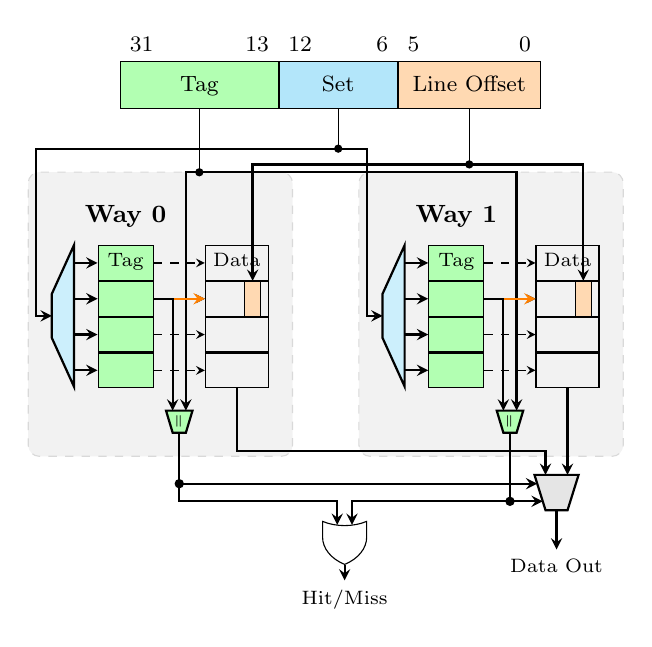
\begin{tikzpicture}[scale=1, transform shape,
    % Style definitions
    addrbox/.style={rectangle, draw, minimum height=0.6cm, font=\footnotesize, text depth=0.1em},
    tagbox/.style={addrbox, fill=green!30, minimum width=2cm},
    setbox/.style={addrbox, fill=cyan!30, minimum width=1.5cm},
    offsetbox/.style={addrbox, fill=orange!30, minimum width=1.8cm},
    cellstyle/.style={rectangle, draw, minimum width=0.7cm, minimum height=0.3cm,
                     text depth=0.1cm, text height=0.2cm, font=\tiny, inner sep=2pt},
    tagcell/.style={cellstyle, fill=green!30},
    datacell/.style={cellstyle, minimum width=0.8cm},
    offsetcell/.style={cellstyle, fill=orange!30, minimum width=2mm},
    decoder/.style={muxdemux, muxdemux def={Lh=1, Rh=3.2, NB=0, NL=1, NR=4, w=0.5, square pins=0},
                   external pins width=0, fill=cyan!20},
    arrow/.style={->, >=stealth, thick},
    dasharrow/.style={dashed, ->, >=stealth},
    orgatestyle/.style={or gate US, draw, logic gate inputs=nn, anchor=center,
                       minimum width=1cm, minimum height=0.8cm, rotate=90},
    junction/.style={circle, fill=black, inner sep=0pt, minimum size=3pt},
    data_connector/.style={circle, fill, inner sep=1.2pt}
]

% Address bits at top - centered
\node[tagbox] at (0,0) (tag) {Tag};
\node[setbox, right=0pt of tag] (set) {Set};
\node[offsetbox, right=0pt of set] (offset) {Line Offset};

% Bit labels above address boxes
\node[anchor=south west, font=\footnotesize] at (tag.north west) {31};
\node[anchor=south east, font=\footnotesize] at (tag.north east) {13};
\node[anchor=south west, font=\footnotesize] at (set.north west) {12};
\node[anchor=south east, font=\footnotesize] at (set.north east) {6};
\node[anchor=south west, font=\footnotesize] at (offset.north west) {5};
\node[anchor=south east, font=\footnotesize] at (offset.north east) {0};

% Way 0 Tag matrix
\matrix[matrix of nodes,
        column sep=0pt, row sep=0pt,
        ampersand replacement=\&,
        anchor=north] at ([xshift=-2.7cm, yshift=-1.6cm]set.south) (tag0) {
  |[tagcell]| {\scriptsize Tag} \\
  |[tagcell]| \phantom{Tag} \\
  |[tagcell]| \phantom{Tag} \\
  |[tagcell]| \phantom{Tag} \\
};

% Way 0 decoder (demux)
\node[decoder, anchor=rpin 1] at ([xshift=-3mm]tag0-1-1.west) (decoder0) {};

% Way 0 Data matrix
\matrix[matrix of nodes,
        column sep=0pt, row sep=0pt,
        ampersand replacement=\&,
        anchor=north west] at ([xshift=4mm]tag0.north east) (data0) {
  |[datacell]| {\scriptsize Data} \\
  |[datacell]| \phantom{Data} \\
  |[datacell]| \phantom{Data} \\
  |[datacell]| \phantom{Data} \\
};
\node[offsetcell, anchor=east] at ([xshift=-1mm]data0-2-1.east) (thedata0) {};

% Way 0 comparator
\node[muxdemux, muxdemux def={Lh=0.6, Rh=0.3, NL=2, NB=1, w=0.5},
      external pins width=0, fill=green!30, rotate=270] at ([xshift=2mm, yshift=-3mm]tag0.south east) (comp0) {};
\node[font=\fontsize{4}{4}\selectfont, rotate=90] at (comp0.center) {=};

% Way 0 label
\node[above=1mm of tag0-1-1.north, font=\small] (way0label) {\textbf{Way 0}};

% Way 1 Tag matrix
\matrix[matrix of nodes,
        column sep=0pt, row sep=0pt,
        ampersand replacement=\&,
        anchor=north] at ([xshift=1.5cm, yshift=-1.6cm]set.south) (tag1) {
  |[tagcell]| {\scriptsize Tag} \\
  |[tagcell]| \phantom{Tag} \\
  |[tagcell]| \phantom{Tag} \\
  |[tagcell]| \phantom{Tag} \\
};

% Way 1 decoder (demux)
\node[decoder, anchor=rpin 1] at ([xshift=-3mm]tag1-1-1.west) (decoder1) {};

% Way 1 Data matrix
\matrix[matrix of nodes,
        column sep=0pt, row sep=0pt,
        ampersand replacement=\&,
        anchor=north west] at ([xshift=4mm]tag1.north east) (data1) {
  |[datacell]| {\scriptsize Data} \\
  |[datacell]| \phantom{Data} \\
  |[datacell]| \phantom{Data} \\
  |[datacell]| \phantom{Data} \\
};
\node[offsetcell, anchor=east] at ([xshift=-1mm]data1-2-1.east) (thedata1) {};

% Way 1 comparator
\node[muxdemux, muxdemux def={Lh=0.6, Rh=0.3, NL=2, NB=1, w=0.5},
      external pins width=0, fill=green!30, rotate=270] at ([xshift=2mm, yshift=-3mm]tag1.south east) (comp1) {};
\node[font=\fontsize{4}{4}\selectfont, rotate=90] at (comp1.center) {=};

% Way 1 label
\node[above=1mm of tag1-1-1.north, font=\small] (way1label) {\textbf{Way 1}};

% Background for ways
\begin{pgfonlayer}{background}
    \node[fit=(way0label)(decoder0)(tag0-1-1)(tag0-4-1)(data0-1-1)(data0-4-1)(comp0),
          fill=gray!10, draw=gray!30, dashed, rounded corners,
          inner sep=3mm] (way0bg) {};
    \node[fit=(way1label)(decoder1)(tag1-1-1)(tag1-4-1)(data1-1-1)(data1-4-1)(comp1),
          fill=gray!10, draw=gray!30, dashed, rounded corners,
          inner sep=3mm] (way1bg) {};
\end{pgfonlayer}

% OR gate
\node[orgatestyle, rotate=180, yscale=0.7, xscale=0.5] at ($(comp0)!0.5!(comp1) + (0,-1.5)$) (orgate) {};

% MUX
\node[muxdemux, muxdemux def={Lh=1, Rh=0.5, NL=2, NB=2, NR=1, w=0.8},
      external pins width=0, fill=gray!20, rotate=270,anchor=lpin 1] at ([yshift=-1.1cm]data1-4-1.south) (mux) {};

% Output labels
\node[below=2mm of orgate.east, font=\scriptsize] (hitmiss) {Hit/Miss};
\node[below=5mm of mux.rpin 1, font=\scriptsize] (dataout) {Data Out};

% Arrows from address bits to decoders with junction
\draw (set.south) -- ++(0,-0.5) coordinate (setjunction);
\node[junction] at (setjunction) {};
\draw[arrow] (setjunction) -| ([xshift=-2mm]decoder0.lpin 1) -- (decoder0.lpin 1);
\draw[arrow] (setjunction) -| ([xshift=-2mm]decoder1.lpin 1) -- (decoder1.lpin 1);

% Arrows from address tag to comparators with junction
\draw (tag.south) -- ++(0,-0.8) coordinate (tagjunction);
\node[junction] at (tagjunction) {};
\draw[arrow] (tagjunction) -| (comp0.lpin 1);
\draw[arrow] (tagjunction) -| (comp1.lpin 1);

% Arrows from offset to data arrays with junction
\draw (offset.south) -- ++(0,-0.7) coordinate (offsetjunction);
\node[junction] at (offsetjunction) {};
\draw[arrow] (offsetjunction) -| (thedata0.north);
\draw[arrow] (offsetjunction) -| (thedata1.north);

% Decoder to tag arrays
\foreach \i in {1,...,4} {
    \draw[arrow] (decoder0.rpin 1 |- tag0-\i-1.west) -- (tag0-\i-1.west);
    \draw[arrow] (decoder1.rpin 1 |- tag1-\i-1.west) -- (tag1-\i-1.west);
}

% Dashed lines from tag arrays to data arrays
\foreach \i in {1,...,4} {
    \draw[dasharrow] (tag0-\i-1.east) -- (data0-\i-1.west);
    \draw[dasharrow] (tag1-\i-1.east) -- (data1-\i-1.west);
}

% Selected line highlighting
\draw[arrow, thick, orange] (tag0-2-1.east) -- (data0-2-1.west);
\draw[arrow, thick, orange] (tag1-2-1.east) -- (data1-2-1.west);

% Tag array output to comparator
\draw[arrow] (tag0-2-1.east) -| (comp0.lpin 2);
\draw[arrow] (tag1-2-1.east) -| (comp1.lpin 2);

% Data array to MUX connections
\draw[arrow] (data0-4-1.south) |- ([yshift=3mm]mux.lpin 2) -- (mux.lpin 2);
\draw[arrow] (data1-4-1.south) -- (mux.lpin 1);

% Comparator outputs to OR gate
\draw[arrow] (comp0.rpin 1) |- ([yshift=3mm]orgate.input 2) -- (orgate.input 2);
\draw[arrow] (comp1.rpin 1) |- ([yshift=3mm]orgate.input 1) -- (orgate.input 1);

% OR gate to Hit/Miss
\draw[arrow] (orgate.output) -- (hitmiss.north);

% Comparator to MUX select
\draw[arrow] (comp0.rpin 1 |- mux.bpin 1) node[data_connector] {} -- (mux.bpin 1);
\draw[arrow] (comp1.rpin 1 |- mux.bpin 2) node[data_connector] {} -- (mux.bpin 2);

% MUX to data out
\draw[arrow] (mux.rpin 1) -- (dataout.north);

\end{tikzpicture}
\end{column}

\begin{column}{0.48\textwidth}
\footnotesize
\begin{tabular}{ll}
\textbf{Line Size:} & $32$ bytes $= 2^5$ bytes\\
\textbf{Cache Size:} & $16$ KB $= 2^{14}$ bytes\\
\textbf{\# Lines:} & $\frac{\text{cache size}}{\text{line size}} = \frac{2^{14}}{2^5} = 512$ lines\\
\textbf{\# Ways:} & $2$\\
\textbf{\# Sets:} & $\frac{\text{\#lines}}{\text{\#ways}} = 256$ sets
\end{tabular}

\vspace{0.2cm}
\begin{tabular}{ll}
\textcolor{offsetcolor}{\textbf{Offset bits:}} & $\log_2(\text{line size}) = 5$ bits\\
\textcolor{setcolor}{\textbf{Set bits:}} & $\log_2(\text{\#sets}) = 8$ bits\\
\textcolor{tagcolor}{\textbf{Tag bits:}} & $32 - (5+8) = 19$ bits\\
\end{tabular}

\vspace{0.3cm}
\textbf{Example:} Address \texttt{0x12345678}\\[2pt]
{\texttt{%
\textcolor{tagcolor}{0001 0010 0011 0100 010}%
\textcolor{setcolor}{1 0110 011}%
\textcolor{offsetcolor}{1 1000}}}\\[4pt]

\footnotesize
\begin{tabular}{ll}
\textcolor{offsetcolor}{\textbf{Offset:}} & \texttt{11000} $= \mathtt{0x18}$\\
\textcolor{setcolor}{\textbf{Set:}} & \texttt{10110011} $= \mathtt{0xB3}$\\
\textcolor{tagcolor}{\textbf{Tag:}} & \texttt{0001001000110100010}\\
                     & $= \mathtt{0x091A2}$\\
\end{tabular}
\end{column}
\end{columns}
\end{frame}


\begin{frame}{2-Way Set Associative vs. Direct Map Cache}

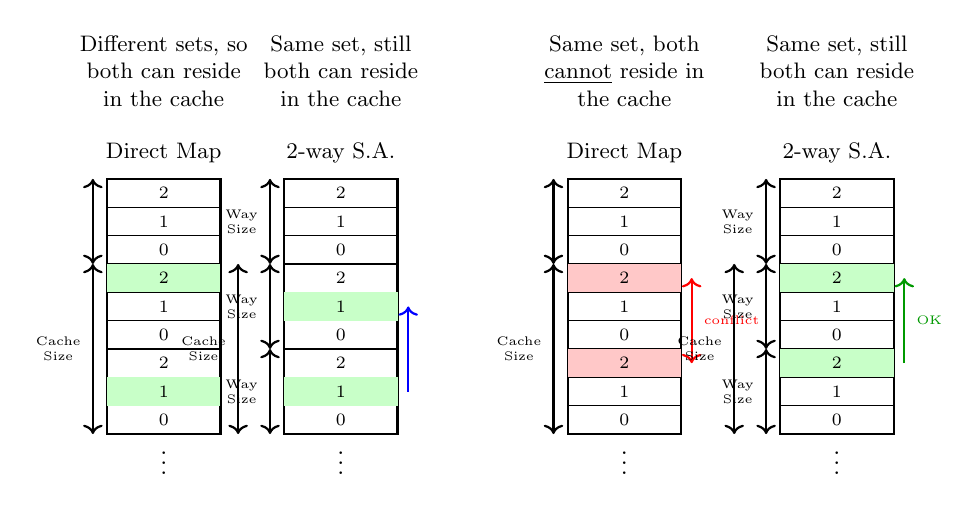
\begin{tikzpicture}[scale=0.9, transform shape]
  % Define colors
  \definecolor{lightgreen}{RGB}{200,255,200}
  \definecolor{lightred}{RGB}{255,200,200}

  % Row height and dimensions
  \def\rowh{0.4}
  \def\colw{1.6}
  \def\nsets{3}  % sets per cache-size or way-size

  % ==================== LEFT GROUP: Different sets - both OK ====================

  % --- Direct Map (different sets) ---
  \begin{scope}[shift={(0,0)}]
    \node[anchor=south, align=center, font=\small] at (\colw/2, 9*\rowh+0.9) {Different sets, so\\both can reside\\in the cache};
    \node[font=\small, anchor=south] at (\colw/2, 9*\rowh+0.1) {Direct Map};

    \draw[thick] (0, 0) rectangle (\colw, 9*\rowh);

    % Draw rows with repeating set numbers (0,1,2,0,1,2,0,1,2)
    \foreach \i in {0, 1, ..., 8} {
      \pgfmathsetmacro{\y}{\i * \rowh}
      \pgfmathtruncatemacro{\setnum}{mod(\i, \nsets)}
      \draw (0, \y) -- (\colw, \y);
      \node[font=\scriptsize] at (\colw/2, \y + \rowh/2) {\setnum};
    }

    % Highlight different sets (green) - row 1 (set 1) and row 5 (set 2)
    \fill[lightgreen] (0, 1*\rowh) rectangle (\colw, 2*\rowh);
    \node[font=\scriptsize] at (\colw/2, 1*\rowh + \rowh/2) {1};
    \fill[lightgreen] (0, 5*\rowh) rectangle (\colw, 6*\rowh);
    \node[font=\scriptsize] at (\colw/2, 5*\rowh + \rowh/2) {2};

    % Cache Size labels (spans 6 rows = twice way size)
    \draw[<->, thick] (-0.2, 0) -- (-0.2, 6*\rowh);
    \node[anchor=east, font=\tiny, align=center] at (-0.25, 3*\rowh) {Cache\\Size};
    \draw[<->, thick] (-0.2, 6*\rowh) -- (-0.2, 9*\rowh);

    \node at (\colw/2, -0.3) {$\vdots$};
  \end{scope}

  % --- 2-way S.A. (different sets) ---
  \begin{scope}[shift={(2.5,0)}]
    \node[anchor=south, align=center, font=\small] at (\colw/2, 9*\rowh+0.9) {Same set, still\\both can reside\\in the cache};
    \node[font=\small, anchor=south] at (\colw/2, 9*\rowh+0.1) {2-way S.A.};

    \draw[thick] (0, 0) rectangle (\colw, 9*\rowh);

    % Draw rows with set numbers repeating (0,1,2,0,1,2,0,1,2)
    \foreach \i in {0, 1, ..., 8} {
      \pgfmathsetmacro{\y}{\i * \rowh}
      \pgfmathtruncatemacro{\setnum}{mod(\i, \nsets)}
      \draw (0, \y) -- (\colw, \y);
      \node[font=\scriptsize] at (\colw/2, \y + \rowh/2) {\setnum};
    }

    % Highlight same set in different ways (green) - row 1 (set 1) and row 4 (set 1)
    \fill[lightgreen] (0, 1*\rowh) rectangle (\colw, 2*\rowh);
    \node[font=\scriptsize] at (\colw/2, 1*\rowh + \rowh/2) {1};
    \fill[lightgreen] (0, 4*\rowh) rectangle (\colw, 5*\rowh);
    \node[font=\scriptsize] at (\colw/2, 4*\rowh + \rowh/2) {1};

    % Arrow connecting same-set rows
    \draw[->, thick, blue] (\colw+0.15, 1.5*\rowh) -- (\colw+0.15, 4.5*\rowh);

    % Way Size labels (inner)
    \foreach \w in {0, 1, 2} {
      \pgfmathsetmacro{\ybot}{\w * 3 * \rowh}
      \pgfmathsetmacro{\ytop}{(\w + 1) * 3 * \rowh}
      \draw[<->, thick] (-0.2, \ybot) -- (-0.2, \ytop);
      \node[anchor=east, font=\tiny, align=center] at (-0.25, \ybot + 1.5*\rowh) {Way\\Size};
    }

    % Cache Size label (outer, spans 6 rows = 2 ways)
    \draw[<->, thick] (-0.65, 0) -- (-0.65, 6*\rowh);
    \node[anchor=east, font=\tiny, align=center] at (-0.7, 3*\rowh) {Cache\\Size};

    \node at (\colw/2, -0.3) {$\vdots$};
  \end{scope}

  % ==================== RIGHT GROUP: Same set - DM conflict, 2-way OK ====================

  % --- Direct Map (same set - CONFLICT) ---
  \begin{scope}[shift={(6.5,0)}]
    \node[anchor=south, align=center, font=\small] at (\colw/2, 9*\rowh+0.9) {Same set, both\\\underline{cannot} reside in\\the cache};
    \node[font=\small, anchor=south] at (\colw/2, 9*\rowh+0.1) {Direct Map};

    \draw[thick] (0, 0) rectangle (\colw, 9*\rowh);

    % Draw rows with repeating set numbers
    \foreach \i in {0, 1, ..., 8} {
      \pgfmathsetmacro{\y}{\i * \rowh}
      \pgfmathtruncatemacro{\setnum}{mod(\i, \nsets)}
      \draw (0, \y) -- (\colw, \y);
      \node[font=\scriptsize] at (\colw/2, \y + \rowh/2) {\setnum};
    }

    % Highlight conflict (red) - two rows mapping to same set (rows 2 and 5, both set 2)
    \fill[lightred] (0, 2*\rowh) rectangle (\colw, 3*\rowh);
    \node[font=\scriptsize] at (\colw/2, 2*\rowh + \rowh/2) {2};
    \fill[lightred] (0, 5*\rowh) rectangle (\colw, 6*\rowh);
    \node[font=\scriptsize] at (\colw/2, 5*\rowh + \rowh/2) {2};

    % Arrow showing conflict between same-set rows
    \draw[<->, thick, red] (\colw+0.15, 2.5*\rowh) -- (\colw+0.15, 5.5*\rowh);
    \node[font=\tiny, red, anchor=west] at (\colw+0.2, 4*\rowh) {conflict};

    % Cache Size labels (spans 6 rows = twice way size)
    \draw[<->, thick] (-0.2, 0) -- (-0.2, 6*\rowh);
    \node[anchor=east, font=\tiny, align=center] at (-0.25, 3*\rowh) {Cache\\Size};
    \draw[<->, thick] (-0.2, 6*\rowh) -- (-0.2, 9*\rowh);

    \node at (\colw/2, -0.3) {$\vdots$};
  \end{scope}

  % --- 2-way S.A. (same set - OK) ---
  \begin{scope}[shift={(9.5,0)}]
    \node[anchor=south, align=center, font=\small] at (\colw/2, 9*\rowh+0.9) {Same set, still\\both can reside\\in the cache};
    \node[font=\small, anchor=south] at (\colw/2, 9*\rowh+0.1) {2-way S.A.};

    \draw[thick] (0, 0) rectangle (\colw, 9*\rowh);

    % Draw rows with set numbers repeating (0,1,2,0,1,2,0,1,2)
    \foreach \i in {0, 1, ..., 8} {
      \pgfmathsetmacro{\y}{\i * \rowh}
      \pgfmathtruncatemacro{\setnum}{mod(\i, \nsets)}
      \draw (0, \y) -- (\colw, \y);
      \node[font=\scriptsize] at (\colw/2, \y + \rowh/2) {\setnum};
    }

    % Highlight same set in different ways (green) - row 2 (set 2) and row 5 (set 2)
    \fill[lightgreen] (0, 2*\rowh) rectangle (\colw, 3*\rowh);
    \node[font=\scriptsize] at (\colw/2, 2*\rowh + \rowh/2) {2};
    \fill[lightgreen] (0, 5*\rowh) rectangle (\colw, 6*\rowh);
    \node[font=\scriptsize] at (\colw/2, 5*\rowh + \rowh/2) {2};

    % Arrow connecting same-set rows (OK because different ways)
    \draw[->, thick, green!60!black] (\colw+0.15, 2.5*\rowh) -- (\colw+0.15, 5.5*\rowh);
    \node[font=\tiny, green!60!black, anchor=west] at (\colw+0.2, 4*\rowh) {OK};

    % Way Size labels (inner)
    \foreach \w in {0, 1, 2} {
      \pgfmathsetmacro{\ybot}{\w * 3 * \rowh}
      \pgfmathsetmacro{\ytop}{(\w + 1) * 3 * \rowh}
      \draw[<->, thick] (-0.2, \ybot) -- (-0.2, \ytop);
      \node[anchor=east, font=\tiny, align=center] at (-0.25, \ybot + 1.5*\rowh) {Way\\Size};
    }

    % Cache Size label (outer, spans 6 rows = 2 ways)
    \draw[<->, thick] (-0.65, 0) -- (-0.65, 6*\rowh);
    \node[anchor=east, font=\tiny, align=center] at (-0.7, 3*\rowh) {Cache\\Size};

    \node at (\colw/2, -0.3) {$\vdots$};
  \end{scope}

\end{tikzpicture}

\vspace{0.15cm}
\small
\begin{itemize}
  \item Memory blocks map to cache sets: set = block\# mod \#sets. Set numbers repeat every cache/way size.
  \item \textbf{Direct-mapped}: blocks mapping to same set $\Rightarrow$ conflict (only one can reside)
  \item \textbf{2-way S.A.}: same set has 2 ways $\Rightarrow$ two blocks can coexist
\end{itemize}

\end{frame}



\begin{frame}[fragile]{LRU Implementation}
\begin{columns}[T]
\begin{column}{0.70\textwidth}
\begin{itemize}
  \item \textcolor{blue}{\textbf{2 ways}}
  \begin{itemize}
    \item 1 bit per set to mark the most recently accessed way in the set
    \item Evict the way which is not pointed to by the bit
  \end{itemize}
  
  \item \textcolor{blue}{\textbf{k-way set associative LRU}}
  \begin{itemize}
    \item For each set maintain the way access order \\
    $\Rightarrow$ per set: log$_2$k bit counter per way
    \begin{itemize}
      \item 4 ways: 4$\times$2 bits per set; 8 ways: 8$\times$3 bits per set
      \item Many bits $\Rightarrow$ complicated update scheme
    \end{itemize}
    \item When way $i$ is accessed: (see next slide)
    \item When replacement is needed: evict the way with counter = 0
  \end{itemize}
\end{itemize}
\end{column}

\begin{column}{0.30\textwidth}
\small
\raggedright
\textbf{Initial State}\\[0.1cm]
\lrutable{0}{1}{2}{3}

\vspace{0.3cm}
\textbf{$\Rightarrow$ Access way 2}\\[0.1cm]
\lrutable{0}{1}{\mru{3}}{\dec{2}}

\vspace{0.3cm}
\textbf{$\Rightarrow$ Access way 0}\\[0.1cm]
\lrutable{\mru{3}}{\dec{0}}{\dec{2}}{\dec{1}}
\end{column}
\end{columns}
\end{frame}

\begin{frame}[fragile]{LRU Implementation -- Update Algorithm}
\begin{columns}[T]
\begin{column}{0.7\textwidth}
\begin{codeboxtitle}{Pseudo-code (on access of way $i$)}
\begin{minted}[fontsize=\small]{python}
X = Counter[i]
Counter[i] = k-1          # way i becomes MRU
for j in range(k):
    if j != i and Counter[j] > X:
        Counter[j] -= 1
\end{minted}
\end{codeboxtitle}

\vspace{0.3cm}
\textbf{Key idea:}
\begin{itemize}
  \item Accessed way gets \mru{highest counter value} ($k-1$)
  \item Other ways with higher counter are \dec{decremented}
  \item Way with counter = 0 is LRU (eviction candidate)
\end{itemize}
\end{column}

\begin{column}{0.3\textwidth}
\small
\raggedright
\textbf{Example (4-way):}\\[0.2cm]

\textbf{Initial State}\\[0.1cm]
\lrutable{0}{1}{2}{3}

\vspace{0.3cm}
\textbf{$\Rightarrow$ Access way 2}\\[0.1cm]
\lrutable{0}{1}{\mru{3}}{\dec{2}}

\vspace{0.3cm}
\textbf{$\Rightarrow$ Access way 0}\\[0.1cm]
\lrutable{\mru{3}}{\dec{0}}{\dec{2}}{\dec{1}}
\end{column}
\end{columns}
\end{frame}

\begin{frame}{Pseudo LRU (PLRU)}
\vspace{-3mm}
\begin{columns}
\begin{column}{0.70\textwidth}
\begin{itemize}
  \item \textbf{PLRU records partial order using tree structure}
  \begin{itemize}
    \item Ways at leaves; PLRU bits at internal nodes
    \item For $n$ leaves: $n-1$ internal nodes (PLRU bits)
  \end{itemize}
  
  \vspace{0.1cm}
  
  \item \textbf{Example: 4-way cache, 3 bits per set}
  \begin{itemize}
    \item Bit$_0$: order between \{0,1\} and \{2,3\}
    \item Bit$_1$: order between ways 0 and 1
    \item Bit$_2$: order between ways 2 and 3
  \end{itemize}
  
  \vspace{0.1cm}
  
  \item \textbf{Update on access:}\\
  Set bits along path to point toward accessed way\\
  {\small \textcolor{orange}{(bit=0 $\Rightarrow$ go left, bit=1 $\Rightarrow$ go right)}}

  \vspace{0.1cm}

  \item \textbf{Victim selection:}\\
  Follow \emph{opposite} of bit values\\
  {\small \textcolor{red!70!black}{(bit=0 $\Rightarrow$ go right, bit=1 $\Rightarrow$ go left)}}

\end{itemize}
\end{column}

\begin{column}{0.28\textwidth}
\centering
\vspace{0.3cm}

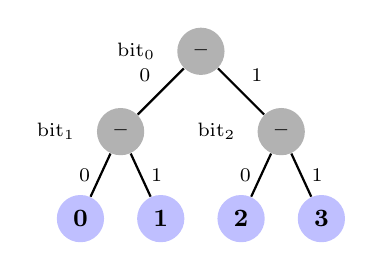
\begin{tikzpicture}[scale=0.85]
  % Tree structure
  \node[circle, fill=gray!60, minimum size=0.6cm, inner sep=0pt, font=\scriptsize\bfseries] (bit0) at (0,0) {--};
  \node[left=0.15cm of bit0, font=\scriptsize] {bit$_0$};

  \node[circle, fill=gray!60, minimum size=0.6cm, inner sep=0pt, font=\scriptsize\bfseries] (bit1) at (-1.2,-1.2) {--};
  \node[left=0.15cm of bit1, font=\scriptsize] {bit$_1$};
  \node[circle, fill=gray!60, minimum size=0.6cm, inner sep=0pt, font=\scriptsize\bfseries] (bit2) at (1.2,-1.2) {--};
  \node[left=0.15cm of bit2, font=\scriptsize] {bit$_2$};

  \node[circle, fill=blue!25, minimum size=0.6cm, inner sep=0pt, font=\small\bfseries] (w0) at (-1.8,-2.5) {0};
  \node[circle, fill=blue!25, minimum size=0.6cm, inner sep=0pt, font=\small\bfseries] (w1) at (-0.6,-2.5) {1};
  \node[circle, fill=blue!25, minimum size=0.6cm, inner sep=0pt, font=\small\bfseries] (w2) at (0.6,-2.5) {2};
  \node[circle, fill=blue!25, minimum size=0.6cm, inner sep=0pt, font=\small\bfseries] (w3) at (1.8,-2.5) {3};

  % Edges with 0/1 labels
  \draw[thick] (bit0) -- (bit1) node[midway, above left, font=\scriptsize] {0};
  \draw[thick] (bit0) -- (bit2) node[midway, above right, font=\scriptsize] {1};
  \draw[thick] (bit1) -- (w0) node[midway, left, font=\scriptsize] {0};
  \draw[thick] (bit1) -- (w1) node[midway, right, font=\scriptsize] {1};
  \draw[thick] (bit2) -- (w2) node[midway, left, font=\scriptsize] {0};
  \draw[thick] (bit2) -- (w3) node[midway, right, font=\scriptsize] {1};
\end{tikzpicture}

\vspace{0.3cm}
\footnotesize
\textbf{Edge labels:}\\
0 = left branch\\
1 = right branch

\vspace{0.3cm}
{\small \textcolor{red}{May not select true LRU}}
\end{column}
\end{columns}
\end{frame}

\begin{frame}{PLRU Example}
\centering
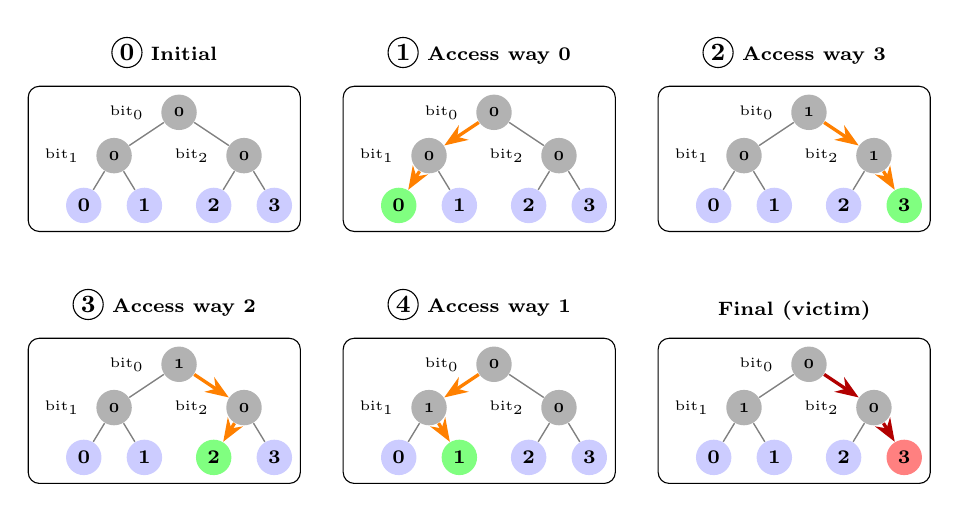
\begin{tikzpicture}[
  treebox/.style={draw, rounded corners, inner sep=3pt, align=center},
  steplabel/.style={font=\scriptsize\bfseries},
]
  % Row 1: Initial, Access 0, Access 3
  \node[treebox] (t0) at (0,0) {\plrutreepath{0}{0}{0}{9}};
  \node[steplabel, above=0.1cm of t0] {\circnum{0} Initial};

  \node[treebox] (t1) at (4,0) {\plrutreepath{0}{0}{0}{0}};
  \node[steplabel, above=0.1cm of t1] {\circnum{1} Access way 0};

  \node[treebox] (t2) at (8,0) {\plrutreepath{1}{0}{1}{3}};
  \node[steplabel, above=0.1cm of t2] {\circnum{2} Access way 3};

  % Row 2: Access 2, Access 1, Final (with victim)
  \node[treebox] (t3) at (0,-3.2) {\plrutreepath{1}{0}{0}{2}};
  \node[steplabel, above=0.1cm of t3] {\circnum{3} Access way 2};

  \node[treebox] (t4) at (4,-3.2) {\plrutreepath{0}{1}{0}{1}};
  \node[steplabel, above=0.1cm of t4] {\circnum{4} Access way 1};

  \node[treebox] (t5) at (8,-3.2) {\plrutreepath{0}{1}{0}{5}};
  \node[steplabel, above=0.1cm of t5] {Final (victim)};
\end{tikzpicture}

\vspace{0.2cm}
\begin{columns}
\begin{column}{0.5\textwidth}
\small
\textbf{Update:} Set bits along \textcolor{orange}{\textbf{path}} to point toward accessed way
\end{column}
\begin{column}{0.5\textwidth}
\small
\textbf{Victim:} Follow \textcolor{green!60!black}{\textbf{opposite}} of arrows → \textcolor{red}{\textbf{Way 3}}
\end{column}
\end{columns}
\end{frame}

\section{Cache Performance}

\begin{frame}{Cache Line Size Trade-offs}
\small
\begin{itemize}
  \item \textbf{Larger lines exploit spatial locality}
  \begin{itemize}
    \item Too big blocks: may fetch unused data
    \item Possibly evicting useful data $\Rightarrow$ miss rate goes up
  \end{itemize}
  \item \textbf{Larger lines mean larger miss penalty}
  \begin{itemize}
    \item Takes longer to perform a cache line fill
    \item Using critical word first reduces the issue
  \end{itemize}
  \item Takes longer to evict (write-back policy)
\end{itemize}
\vspace{0.2cm}
\centering
\includegraphics[height=3cm]{figures/cache_line_size_tradeoff.png}
\vspace{0.2cm}

$t_{\text{avg}} = t_{hit}\times(1-\text{MR}) + t_{miss}\times \text{MR}$
\end{frame}


\begin{frame}{Effect of Cache on Performance}

\begin{itemize}
  \item \textbf{MPI — misses per instruction}
  \begin{itemize}
    \item MPI = $\frac{\text{\#cache misses}}{\text{\#instructions}} = \frac{\text{\#cache misses}}{\text{\#mem accesses}} \times \frac{\text{\#mem accesses}}{\text{\#instructions}}$
    \item More correlative to performance than cache miss rate
    \begin{itemize}
      \item Takes into account also frequency of memory accesses
    \end{itemize}
  \end{itemize}
  
  \vspace{0.4cm}
  
  \item[\textcolor{blue}{$\diamond$}] \textbf{Memory stall cycles}
  \begin{itemize}
    \item[] = \#memory accesses $\times$ miss rate $\times$ miss penalty
    \item[] = IC $\times$ MPI $\times$ miss penalty
  \end{itemize}
  
  \vspace{0.4cm}
  
  \item[\textcolor{blue}{$\diamond$}] \textbf{CPU time}
  \begin{itemize}
    \item[] = (CPU execution cycles + Memory stall cycles) $\times$ cycle time
    \item[] = IC $\times$ (CPI$_{\text{execution}}$ + MPI $\times$ Miss penalty) $\times$ cycle time
  \end{itemize}
\end{itemize}

\end{frame}

\begin{frame}{Classifying Misses: The 3Cs}
\begin{columns}[T]
\begin{column}{0.52\textwidth}
\small
\begin{itemize}
  \item \textbf{Compulsory}: first reference to a block
  \begin{itemize}\scriptsize
    \item Solution: prefetch
  \end{itemize}
  \item \textbf{Capacity}: working set $>$ cache size
  \begin{itemize}\scriptsize
    \item Solution: increase size, stream buffers
  \end{itemize}
  \item \textbf{Conflict}: set mapping causes evictions
  \begin{itemize}\scriptsize
    \item Solution: higher associativity, victim cache
  \end{itemize}
\end{itemize}
\end{column}
\begin{column}{0.48\textwidth}
\centering
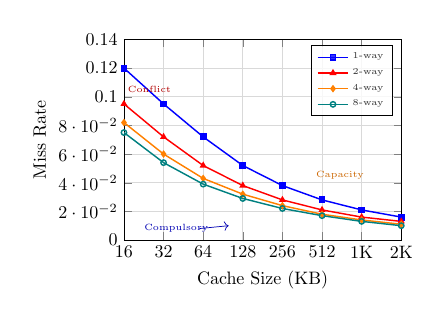
\begin{tikzpicture}[scale=0.65]
\begin{axis}[
    xlabel={Cache Size (KB)},
    ylabel={Miss Rate},
    xmode=log,
    log basis x=2,
    xmin=16, xmax=2048,
    ymin=0, ymax=0.14,
    xtick={16,32,64,128,256,512,1024,2048},
    xticklabels={16,32,64,128,256,512,1K,2K},
    ytick={0,0.02,0.04,0.06,0.08,0.10,0.12,0.14},
    legend pos=north east,
    legend style={font=\tiny, fill=white, fill opacity=0.8},
    grid=major,
    grid style={gray!30},
    width=7cm,
    height=5.5cm,
]
% 1-way (highest miss rate)
\addplot[blue, thick, mark=square*, mark size=1.5pt] coordinates {
    (16,0.12) (32,0.095) (64,0.072) (128,0.052) (256,0.038) (512,0.028) (1024,0.021) (2048,0.016)
};
% 2-way
\addplot[red, thick, mark=triangle*, mark size=1.5pt] coordinates {
    (16,0.095) (32,0.072) (64,0.052) (128,0.038) (256,0.028) (512,0.021) (1024,0.016) (2048,0.013)
};
% 4-way
\addplot[orange, thick, mark=diamond*, mark size=1.5pt] coordinates {
    (16,0.082) (32,0.060) (64,0.043) (128,0.032) (256,0.024) (512,0.018) (1024,0.014) (2048,0.011)
};
% 8-way
\addplot[teal, thick, mark=o, mark size=1.5pt] coordinates {
    (16,0.075) (32,0.054) (64,0.039) (128,0.029) (256,0.022) (512,0.017) (1024,0.013) (2048,0.010)
};
\legend{1-way, 2-way, 4-way, 8-way}

% Annotations for miss types
\node[font=\tiny, blue!70!black] at (axis cs:40,0.008) {Compulsory};
\draw[<-, thin, blue!70!black] (axis cs:100,0.010) -- (axis cs:60,0.008);
\node[font=\tiny, orange!80!black] at (axis cs:700,0.045) {Capacity};
\node[font=\tiny, red!70!black] at (axis cs:25,0.105) {Conflict};
\end{axis}
\end{tikzpicture}
\end{column}
\end{columns}
\end{frame}

\section{Cache Optimization Techniques}

\begin{frame}{Fill Buffers}
\begin{columns}[T]
\begin{column}{0.48\textwidth}
\begin{itemize}
  \item L2 to L1 bus may be narrower than cache line
  \begin{itemize}
    \item E.g., 16B bus, 64B line $\Rightarrow$ 4 cycles
    \item Fetch critical chunk first to reduce latency
  \end{itemize}
  \item Fill buffer accumulates full line, then writes to L1
  \item Streaming loads: bypass L1 to avoid pollution
\end{itemize}
\end{column}
\begin{column}{0.48\textwidth}
\centering
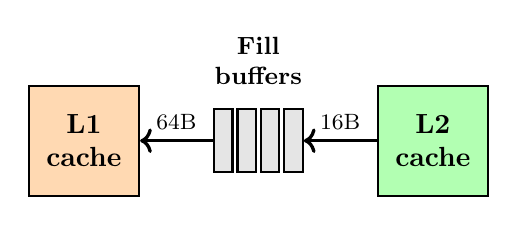
\begin{tikzpicture}[
    cache/.style={draw, thick, minimum width=1.4cm, minimum height=1.4cm, inner sep=2pt, align=center, font=\bfseries},
    buffer/.style={draw, thick, minimum width=0.175cm, minimum height=0.8cm},
    ]

    % L1 cache (left)
    \node[cache, fill=orange!30] (l1) at (0, 0) {L1\\cache};

    % Fill buffers (center) as matrix - horizontal cells (columns)
    \matrix[right=0.8cm of l1, matrix of nodes,
            nodes={buffer, fill=gray!20},
            column sep=1pt, ampersand replacement=\&] (fillbuf) {
        |(b1)| \& |(b2)| \& |(b3)| \& |(b4)| \\
    };

    % Label for fill buffers (above)
    \node[above=0.5mm of fillbuf, font=\small\bfseries, align=center] {Fill\\buffers};

    % L2 cache (right)
    \node[cache, fill=green!30, right=0.8cm of fillbuf] (l2) {L2\\cache};

    % Arrows (data flows from L2 -> buffers -> L1)
    \draw[->, very thick] (l2.west |- b4.east) -- node[above, font=\footnotesize] {16B} (b4.east);
    \draw[->, very thick] (b1.west) -- node[above, font=\footnotesize] {64B} (b1.west -| l1.east);
\end{tikzpicture}

\vspace{0.4cm}
\begin{itemize}
  \item Typically 4--8 entries
  \item Searched in parallel with cache
  \item Can forward data before fill completes
  \item Enables hit-under-miss
\end{itemize}
\end{column}
\end{columns}
\end{frame}






\begin{frame}{Victim Cache}
\begin{columns}[T]
\begin{column}{0.48\textwidth}\small
\textbf{Victim cache gives a 2\textsuperscript{nd} chance to evicted lines}
\begin{itemize}\small
  \item \circnum{1} A line evicted from L1 cache is placed in the Victim Cache
  \item \circnum{2} If the Victim Cache is full $\Rightarrow$ evict its LRU line to the L2 cache
  \item Victim cache is small and can be built as fully associative
\end{itemize}
\vspace{0.3cm}
\textbf{On L1 cache lookup, lookup the Victim Cache in parallel}
\end{column}
\begin{column}{0.48\textwidth}
\centering
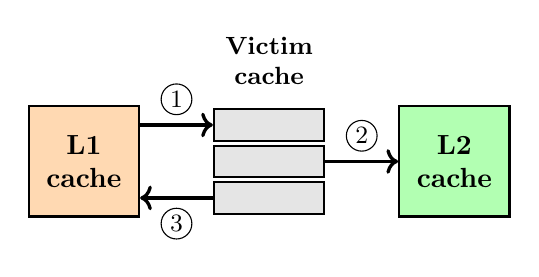
\begin{tikzpicture}[
    cache/.style={draw, thick, minimum width=1.4cm, minimum height=1.4cm, inner sep=2pt, align=center, font=\bfseries},
    vcache/.style={draw, thick, minimum width=1.4cm, minimum height=0.4cm},
    ]

    % L1 cache (left)
    \node[cache, fill=orange!30] (l1) at (0, 0) {L1\\cache};

    % Victim cache (center) as matrix
    \matrix[right=0.8cm of l1, matrix of nodes,
            nodes={vcache, fill=gray!20},
            row sep=1pt] (victim) {
        |(v1)| \\
        |(v2)| \\
        |(v3)| \\
    };

    % Label for victim cache (above, closer)
    \node[above=0.5mm of victim, font=\small\bfseries, align=center] {Victim\\cache};

    % L2 cache (right)
    \node[cache, fill=green!30, right=0.8cm of victim] (l2) {L2\\cache};

    % Arrows
    \draw[->, very thick] (l1.east |- v1.west) -- node[above, font=\small] {\circnum{1}} (v1.west);
    \draw[->, very thick] (v2.east) -- node[above, font=\small] {\circnum{2}} (v2.east -| l2.west);
    \draw[->, very thick] (v3.west) -- node[below, font=\small] {\circnum{3}} (v3.west -| l1.east);
\end{tikzpicture}

\vspace{0.2cm}
\small
\begin{itemize}\small
  \item Data supplied to the core directly from Victim Cache at same access time as L1 cache hit
  \item \circnum{3} On victim cache hit move the line back from the Victim Cache into the L1 cache
  \begin{itemize}\scriptsize
    \item Evicted line moved to the Victim Cache
  \end{itemize}
\end{itemize}
\end{column}
\end{columns}
\end{frame}

\begin{frame}{Memory Updates on Writes}
\begin{columns}[T]
\column{0.5\textwidth}
\textbf{Write-back --- cheaper writes}
\begin{itemize}
  \item Store hits write only to cache
  \begin{itemize}
    \item Memory not accessed on write hit
    \item Line marked as \emph{dirty}
  \end{itemize}
  \item Dirty line written to memory only on eviction
  \begin{itemize}
    \item Saves accesses when line updated many times
    \item Must write entire line (no per-byte tracking)
  \end{itemize}
\end{itemize}
\column{0.5\textwidth}
\textbf{Write-through --- cheaper evictions}
\begin{itemize}
  \item Store hits write to cache \emph{and} memory
  \begin{itemize}
    \item Only changed bytes written (not entire line)
  \end{itemize}
  \item Reads:writes ratio $\approx$ 4:1
  \begin{itemize}
    \item Processor reads from cache while write proceeds
  \end{itemize}
  \item No dirty lines $\Rightarrow$ evictions are free
  \item Uses write buffer to hide memory latency
\end{itemize}
\end{columns}
\end{frame}

\begin{frame}{Write Buffer \& Write Combining}
\begin{columns}[T]
\begin{column}{0.55\textwidth}
\begin{itemize}
  \item Buffer decouples CPU stores from DRAM writes
  \item Combine multiple writes to same line into one buffer entry
  \item On a miss, also consult write buffer for the most up-to-date bytes
\end{itemize}
\end{column}
\begin{column}{0.42\textwidth}
\centering
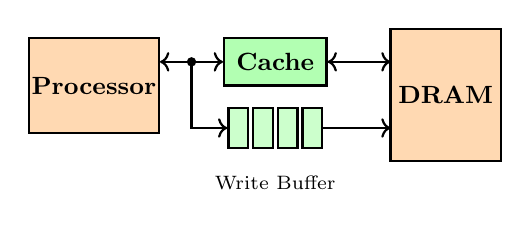
\begin{tikzpicture}[
    procbox/.style={draw, thick, minimum width=1.3cm, minimum height=1.2cm, inner sep=1pt, align=center, font=\small\bfseries},
    cachebox/.style={draw, thick, minimum width=1.3cm, minimum height=0.6cm, inner sep=1pt, align=center, font=\small\bfseries},
    wbuf/.style={draw, thick, minimum width=0.25cm, minimum height=0.5cm, fill=green!20},
    data_connector/.style={circle, fill, inner sep=1.2pt},
    ]
    % DRAM as mux (anchor point for positioning)
    \node[muxdemux, muxdemux def={Lh=3, Rh=3, NL=2, NR=0, NB=0, NT=0, w=2.5},
          external pins width=0, fill=orange!30, font=\small\bfseries] (dram) {DRAM};

    % Cache positioned relative to DRAM lpin 1
    \node[cachebox, fill=green!30, left=0.8cm of dram.lpin 1] (cache) {Cache};

    % Processor (taller, same height as DRAM)
    \node[procbox, fill=orange!30, anchor=north east] (proc) at ([xshift=-8mm]cache.north west) {Processor};

    % Write buffer positioned relative to DRAM lpin 2
    \matrix[matrix of nodes, nodes={wbuf},
            column sep=1pt, ampersand replacement=\&] (wbuf) at (dram.lpin 2 -| cache) {
        |(w1)| \& |(w2)| \& |(w3)| \& |(w4)| \\
    };
    \node[below=1mm of wbuf, font=\scriptsize] {Write Buffer};

    % Arrows (all thick)
    \draw[<->, thick] (proc.east |- cache) -- (cache);
    \draw[<->, thick] (cache) -- (dram.lpin 1);
    \draw[->, thick] (w4.east) -- (dram.lpin 2);

    % Data connector from proc-cache line down to write buffer
    \draw[->, thick] ([xshift=4mm]proc.east |- cache) node[data_connector] (junc) {} |- (w1.west);
\end{tikzpicture}
\end{column}
\end{columns}
\end{frame}

\begin{frame}{Cache Write Miss}
\begin{itemize}
  \item \textbf{The processor is not waiting for data}
  \begin{itemize}
    \item[$\Rightarrow$] continues its work
  \end{itemize}
  
  \vspace{0.5cm}
  
  \item \textbf{Option 1: Write-allocate: fetch the write miss line into the cache}
  \begin{itemize}
    \item[\textcolor{green}{$\checkmark$}] Goes with \textit{write back} policy, assuming more writes are needed
    \item[\textcolor{green}{$\checkmark$}] Hoping that subsequent writes to the line hit the cache
  \end{itemize}
  
  \vspace{0.5cm}
  
  \item \textbf{Option 2: Write-no-allocate: do not fetch the write miss line into the cache}
  \begin{itemize}
    \item[\textcolor{green}{$\checkmark$}] Goes with \textit{write through} policy
    \item[\textcolor{green}{$\checkmark$}] Subsequent writes would update memory anyhow
  \end{itemize}
\end{itemize}
\end{frame}

\newcommand{\prefetchTextCol}{0.7\textwidth}
\newcommand{\prefetchFigCol}{0.3\textwidth}
\newcommand{\prefetchLooseness}{2.5}

\begin{frame}{Hardware Data Prefetching}
\textbf{Predict future data accesses based on observed patterns}
% Streaming prefetcher
\begin{columns}[T]
\begin{column}{\prefetchTextCol}
\begin{itemize}
  \item \textbf{Streaming prefetcher}
  \begin{itemize}
    \item Triggered by ascending access to recent data
    \item Fetches next sequential line(s)
  \end{itemize}
\end{itemize}
\end{column}
\begin{column}{\prefetchFigCol}
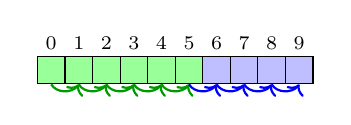
\begin{tikzpicture}[baseline=(current bounding box.center),
  idx/.style={minimum width=0.35cm, font=\scriptsize, inner sep=0pt},
  cell/.style={draw, minimum width=0.35cm, minimum height=0.35cm, inner sep=0pt},
  acc/.style={cell, fill=green!40},
  pref/.style={cell, fill=blue!25},
  gacc/.style={->, thick, green!60!black, looseness=\prefetchLooseness, out=-60, in=-120},
  gpref/.style={->, thick, blue, looseness=\prefetchLooseness, out=-60, in=-120},
]
\matrix[matrix of nodes, column sep=-\pgflinewidth, row sep=0.08cm, ampersand replacement=\&] (m) {
  |[idx]| 0 \& |[idx]| 1 \& |[idx]| 2 \& |[idx]| 3 \& |[idx]| 4 \& |[idx]| 5 \& |[idx]| 6 \& |[idx]| 7 \& |[idx]| 8 \& |[idx]| 9 \\
  |[acc]| \phantom{0} \& |[acc]| \phantom{0} \& |[acc]| \phantom{0} \& |[acc]| \phantom{0} \& |[acc]| \phantom{0} \& |[acc]| \phantom{0} \& |[pref]| \phantom{0} \& |[pref]| \phantom{0} \& |[pref]| \phantom{0} \& |[pref]| \phantom{0} \\
};
\draw[gacc] (m-2-1.south) to (m-2-2.south);
\draw[gacc] (m-2-2.south) to (m-2-3.south);
\draw[gacc] (m-2-3.south) to (m-2-4.south);
\draw[gacc] (m-2-4.south) to (m-2-5.south);
\draw[gacc] (m-2-5.south) to (m-2-6.south);
\draw[gpref] (m-2-6.south) to (m-2-7.south);
\draw[gpref] (m-2-7.south) to (m-2-8.south);
\draw[gpref] (m-2-8.south) to (m-2-9.south);
\draw[gpref] (m-2-9.south) to (m-2-10.south);
\end{tikzpicture}
\end{column}
\end{columns}

\vspace{4mm}

% Stride prefetcher
\begin{columns}[T]
\begin{column}{\prefetchTextCol}
\begin{itemize}
  \item \textbf{Stride prefetcher}
  \begin{itemize}
    \item Tracks loads, detects regular stride
    \item Prefetch = current addr + stride
  \end{itemize}
\end{itemize}
\end{column}
\begin{column}{\prefetchFigCol}
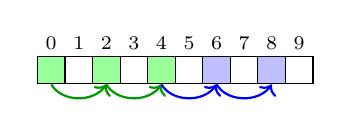
\begin{tikzpicture}[baseline=(current bounding box.center),
  idx/.style={minimum width=0.35cm, font=\scriptsize, inner sep=0pt},
  cell/.style={draw, minimum width=0.35cm, minimum height=0.35cm, inner sep=0pt},
  acc/.style={cell, fill=green!40},
  pref/.style={cell, fill=blue!25},
  gacc/.style={->, thick, green!60!black, looseness=\prefetchLooseness, out=-60, in=-120},
  gpref/.style={->, thick, blue, looseness=\prefetchLooseness, out=-60, in=-120},
]
\matrix[matrix of nodes, column sep=-\pgflinewidth, row sep=0.08cm, ampersand replacement=\&] (m) {
  |[idx]| 0 \& |[idx]| 1 \& |[idx]| 2 \& |[idx]| 3 \& |[idx]| 4 \& |[idx]| 5 \& |[idx]| 6 \& |[idx]| 7 \& |[idx]| 8 \& |[idx]| 9 \\
  |[acc]| \phantom{0} \& |[cell]| \phantom{0} \& |[acc]| \phantom{0} \& |[cell]| \phantom{0} \& |[acc]| \phantom{0} \& |[cell]| \phantom{0} \& |[pref]| \phantom{0} \& |[cell]| \phantom{0} \& |[pref]| \phantom{0} \& |[cell]| \phantom{0} \\
};
\draw[gacc] (m-2-1.south) to (m-2-3.south);
\draw[gacc] (m-2-3.south) to (m-2-5.south);
\draw[gpref] (m-2-5.south) to (m-2-7.south);
\draw[gpref] (m-2-7.south) to (m-2-9.south);
\end{tikzpicture}
\end{column}
\end{columns}

\vspace{4mm}

% General pattern prefetcher
\begin{columns}[T]
\begin{column}{\prefetchTextCol}
\begin{itemize}
  \item \textbf{General pattern prefetcher}
  \begin{itemize}
    \item Identifies patterns in address distances
  \end{itemize}
\end{itemize}
\end{column}
\begin{column}{\prefetchFigCol}
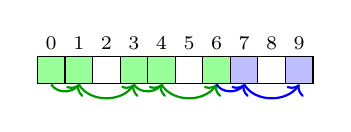
\begin{tikzpicture}[baseline=(current bounding box.center),
  idx/.style={minimum width=0.35cm, font=\scriptsize, inner sep=0pt},
  cell/.style={draw, minimum width=0.35cm, minimum height=0.35cm, inner sep=0pt},
  acc/.style={cell, fill=green!40},
  pref/.style={cell, fill=blue!25},
  gacc/.style={->, thick, green!60!black, looseness=\prefetchLooseness, out=-60, in=-120},
  gpref/.style={->, thick, blue, looseness=\prefetchLooseness, out=-60, in=-120},
]
\matrix[matrix of nodes, column sep=-\pgflinewidth, row sep=0.08cm, ampersand replacement=\&] (m) {
  |[idx]| 0 \& |[idx]| 1 \& |[idx]| 2 \& |[idx]| 3 \& |[idx]| 4 \& |[idx]| 5 \& |[idx]| 6 \& |[idx]| 7 \& |[idx]| 8 \& |[idx]| 9 \\
  |[acc]| \phantom{0} \& |[acc]| \phantom{0} \& |[cell]| \phantom{0} \& |[acc]| \phantom{0} \& |[acc]| \phantom{0} \& |[cell]| \phantom{0} \& |[acc]| \phantom{0} \& |[pref]| \phantom{0} \& |[cell]| \phantom{0} \& |[pref]| \phantom{0} \\
};
\draw[gacc] (m-2-1.south) to (m-2-2.south);
\draw[gacc] (m-2-2.south) to (m-2-4.south);
\draw[gacc] (m-2-4.south) to (m-2-5.south);
\draw[gacc] (m-2-5.south) to (m-2-7.south);
\draw[gpref] (m-2-7.south) to (m-2-8.south);
\draw[gpref] (m-2-8.south) to (m-2-10.south);
\end{tikzpicture}
\end{column}
\end{columns}

\vspace{0mm}

% DMP prefetcher
\begin{columns}[T]
\begin{column}{\prefetchTextCol}
\begin{itemize}
  \item \textbf{Data memory-dependent (DMP)}
  \begin{itemize}
    \item Examines data values in cache
    \item Values that look like pointers trigger prefetch
  \end{itemize}
\end{itemize}
\end{column}
\begin{column}{\prefetchFigCol}
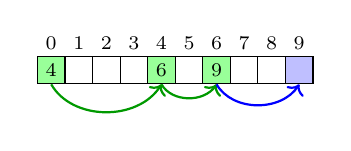
\begin{tikzpicture}[baseline=(current bounding box.center),
  idx/.style={minimum width=0.35cm, font=\scriptsize, inner sep=0pt},
  cell/.style={draw, minimum width=0.35cm, minimum height=0.35cm, font=\scriptsize, inner sep=0pt},
  acc/.style={cell, fill=green!40},
  pref/.style={cell, fill=blue!25},
  gacc/.style={->, thick, green!60!black, looseness=\prefetchLooseness, out=-60, in=-120},
  gpref/.style={->, thick, blue, looseness=\prefetchLooseness, out=-60, in=-120},
]
\matrix[matrix of nodes, column sep=-\pgflinewidth, row sep=0.08cm, ampersand replacement=\&] (m) {
  |[idx]| 0 \& |[idx]| 1 \& |[idx]| 2 \& |[idx]| 3 \& |[idx]| 4 \& |[idx]| 5 \& |[idx]| 6 \& |[idx]| 7 \& |[idx]| 8 \& |[idx]| 9 \\
  |[acc]| 4 \& |[cell]| \phantom{0} \& |[cell]| \phantom{0} \& |[cell]| \phantom{0} \& |[acc]| 6 \& |[cell]| \phantom{0} \& |[acc]| 9 \& |[cell]| \phantom{0} \& |[cell]| \phantom{0} \& |[pref]| \phantom{0} \\
};
\draw[gacc] (m-2-1.south) to (m-2-5.south);
\draw[gacc] (m-2-5.south) to (m-2-7.south);
\draw[gpref] (m-2-7.south) to (m-2-10.south);
\end{tikzpicture}
\end{column}
\end{columns}

\vspace{0.1em}
\hfill{\scriptsize\color{gray} {\color{green!60!black}$\blacksquare$} accessed \quad {\color{blue!50}$\blacksquare$} prefetched}
\end{frame}

\begin{frame}{Prefetching: Timing and Trade-offs}
\begin{itemize}
  \item \textbf{Data must be prefetched before it is needed}
  \begin{itemize}
    \item The prefetcher aggressiveness has to be tuned
    \item How fast and how far ahead to issue requests, so data arrives on time
  \end{itemize}

  \item \textbf{Prefetching relies on extra memory bandwidth}
  \begin{itemize}
    \item Too aggressive/inaccurate prefetching slows demand fetches and pollutes cache
  \end{itemize}

  \item \textbf{Software Prefetching}
  \begin{itemize}
    \item Special prefetching instructions that cannot cause faults
  \end{itemize}

  \item \textbf{Instruction Prefetching}
  \begin{itemize}
    \item On a cache miss, prefetch sequential cache lines into stream buffers
    \item Branch predictor directed prefetching -- let predictor run ahead
  \end{itemize}
\end{itemize}
\end{frame}

\begin{frame}{Code Optimizations for Locality}
We will explore three compiler/programmer techniques to improve cache behavior:
\begin{itemize}
  \item \textbf{Merging arrays}: AoS vs SoA trade-offs; reduce conflicts, improve spatial locality
  \item \textbf{Loop fusion}: combine loops with same traversal to increase reuse
  \item \textbf{Loop interchange}: access arrays in memory order to exploit spatial locality
\end{itemize}
\end{frame}



\begin{frame}[fragile]{Code Optimizations: Merging Arrays}
\begin{itemize}
  \item \textbf{Merge 2 arrays into a single array of compound elements}
\end{itemize}

\begin{columns}
\begin{column}{0.65\textwidth}
\begin{codeboxtitle}{Before: two sequential arrays}
\begin{minted}[fontsize=\small]{c}
int val[SIZE];
int key[SIZE];
\end{minted}
\end{codeboxtitle}

\begin{codeboxtitle}{After: One array of structures}
\begin{minted}[fontsize=\small]{c}
struct merge {
    int val;
    int key;
} merged_array[SIZE];
\end{minted}
\end{codeboxtitle}
\end{column}

\begin{column}{0.35\textwidth}
\begin{itemize}
  \item Reduces conflicts between val and key
  \item Improves spatial locality
\end{itemize}
\end{column}
\end{columns}
\end{frame}

\begin{frame}[fragile]{Code Optimizations: Loop Fusion}
\begin{itemize}
  \item \textbf{Merge loops with shared data access}
  \item Assume each element in \texttt{a} is 4 bytes, 32KB cache, 32 B/line
\end{itemize}

\begin{columns}
\begin{column}{0.55\textwidth}
\begin{codeboxtitle}{Before Fusion}
\begin{minted}[fontsize=\small]{c}
for (i = 0; i < 10000; i++)
  a[i] = 1 / a[i];
for (i = 0; i < 10000; i++)
  sum = sum + a[i];
\end{minted}
\end{codeboxtitle}

\vspace{0.2cm}
\begin{codeboxtitle}{After Fusion}
\begin{minted}[fontsize=\small]{c}
for (i = 0; i < 10000; i++) {
  a[i] = 1 / a[i];
  sum = sum + a[i];
}
\end{minted}
\end{codeboxtitle}
\end{column}

\begin{column}{0.45\textwidth}
\textbf{Before Fusion:}
\begin{itemize}
  \item First loop: hit in 7/8 of iterations
  \item Second loop: array $>$ cache $\Rightarrow$ same hit rate
\end{itemize}

\vspace{0.5cm}
\textbf{After Fusion:}
\begin{itemize}
  \item First line: hit in 7/8 of iterations
  \item Second line: hit in all iterations
\end{itemize}

\vspace{0.2cm}
\footnotesize
\textit{Note: Only load accesses considered for hit rate}
\end{column}
\end{columns}
\end{frame}

\begin{frame}[fragile]{Code Optimizations: Loop Interchange}
\small
\textbf{2D array in memory:}
\texttt{x[0][0] x[0][1] ... x[0][99] x[1][0] x[1][1] ...}

\vspace{0.2cm}
\begin{codeboxtitle}{Original program: accesses are 100 bytes apart}
\begin{minted}[fontsize=\footnotesize]{c}
/* x[0][0] x[1][0] ... x[4999][0] x[0][1] ... */
for (j = 0; j < 100; j++)
  for (i = 0; i < 5000; i++)
    x[i][j] = 2 * x[i][j];
\end{minted}
\end{codeboxtitle}

\vspace{0.15cm}
\begin{codeboxtitle}{Reversing the loop order: accesses are adjacent}
\begin{minted}[fontsize=\footnotesize,escapeinside=??]{c}
/* Improved spatial locality */
for (i = 0; i < 5000; i++)  ?\tikzmarknode{forI}{\strut}?
  for (j = 0; j < 100; j++)  ?\tikzmarknode{forJ}{\strut}?
    x[i][j] = 2 * x[i][j];
\end{minted}
\end{codeboxtitle}

\makeatletter
\@ifundefined{pgf@sh@nt@forI}{}{%
\@ifundefined{pgf@sh@nt@forJ}{}{%
\begin{tikzpicture}[remember picture, overlay]
    \draw[<->, thick, green!70!black, line width=1.2pt]
      ([xshift=5pt]forI.east) to[out=0, in=0, looseness=2.5]
      node[right, font=\scriptsize, pos=0.5] {swap}
      ([xshift=5pt]forJ.east -| forI);
\end{tikzpicture}%
}}
\makeatother
\end{frame}

\begin{frame}{Improving Cache Performance (summary)}
\begin{itemize}
  \item \textbf{Reduce miss rate}: bigger caches/lines, higher associativity, victim cache, stream buffers, prefetching, compiler transforms
  \item \textbf{Reduce miss penalty}: early restart/critical word first, non-blocking caches, L2/L3
  \item \textbf{Reduce hit time}: smaller, on-chip, direct-mapped L1
\end{itemize}
\end{frame}

\section{Advanced Cache Topics}

\begin{frame}{Split I-Cache / D-Cache}
\begin{itemize}
  \item Parallel fetch and data access in different pipeline stages
  \item Different characteristics: I$:$ read-only; D$:$ reads and writes; different prefetching
  \item Self-modifying code: snoop I-cache tags and invalidate on matching store
\end{itemize}
\end{frame}

\begin{frame}{Non-Blocking Caches}
\begin{itemize}
  \item \textbf{Hit Under Miss}
  \begin{itemize}
    \item Allow cache hits while one miss is in progress
    \item Another miss has to wait
    \item Relevant for an out-of-order execution CPU
  \end{itemize}
  \vspace{0.2cm}
  \item \textbf{Miss Under Miss, Hit Under Multiple Misses}
  \begin{itemize}
    \item Allow hits and misses when other misses in progress
    \item Memory system must allow multiple pending requests
    \item Manage a list of outstanding cache misses
    \begin{itemize}
      \item When miss is served and data gets back, update list
    \end{itemize}
  \end{itemize}
\end{itemize}
\end{frame}

\begin{frame}{Multi-ported / Banked Caches}
\begin{itemize}
  \item True $n$-ported caches enable $n$ parallel accesses but nearly double the area
  \item Alternative: \textbf{banked} caches to allow some parallel accesses with less cost
\end{itemize}
\end{frame}

\begin{frame}{L2 Cache (and beyond)}
\begin{itemize}
  \item Larger but slower; reduces L1 miss penalty by filtering DRAM
  \item Often shared across cores; may be \textbf{inclusive} of all L1s
  \item Inclusive L2 must snoop/invalidate L1s on L2 evictions
\end{itemize}
\end{frame}

\section{Cache Coherence}

\begin{frame}{Coherence Basics}
\begin{itemize}
  \item Coherent if: (1) a later read returns the last written value; (2) all processors see stores to the same address in the same order
\end{itemize}
\end{frame}

\begin{frame}{MESI Protocol: States}
\begin{center}
\begin{tabular}{lccc}
\toprule
State & Valid & Modified & Copies elsewhere?\\
\midrule
Invalid   & No  & N/A  & possibly\\
Shared    & Yes & No   & possibly\\
Exclusive & Yes & No   & No\\
Modified  & Yes & Yes  & No\\
\bottomrule
\end{tabular}
\end{center}
\begin{itemize}
  \item To modify, a core must first obtain \textbf{ownership} (no other sharers).
\end{itemize}
\end{frame}

\begin{frame}{MESI Protocol: Actions}
\centering
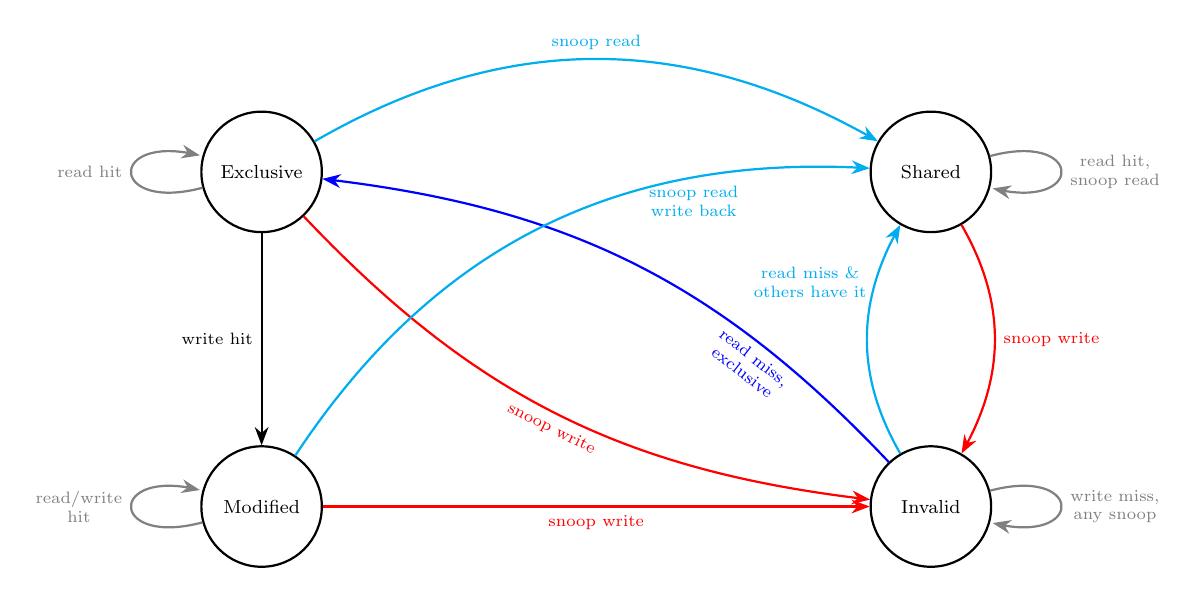
\begin{tikzpicture}[scale=0.85, transform shape,
    state/.style={circle, draw, minimum size=1.8cm, thick, font=\footnotesize},
    arrow/.style={->, >=Stealth, thick},
    %every edge/.style={arrow},
    auto,
    node distance=3.5cm
]

% Define states - closer together
\node[state] (invalid) at (0,0) {Invalid};
\node[state] (shared) at (0,5) {Shared};
\node[state] (exclusive) at (-10,5) {Exclusive};
\node[state] (modified) at (-10,0) {Modified};

% Self-loops - only one per state
\path[arrow]
    (invalid) edge[loop right, gray]node[font=\scriptsize, align=center, anchor=west] {write miss,\\any snoop} (invalid)
    (shared) edge[loop right, gray] node[font=\scriptsize, align=center, anchor=west] {read hit,\\snoop read} (shared)
    (exclusive) edge[loop left, gray] node[font=\scriptsize] {read hit} (exclusive)
    (modified) edge[loop left, gray] node[font=\scriptsize, align=center] {read/write\\hit} (modified);

% Transitions between states - all unidirectional with better separation
\path[arrow]
    % From Invalid
    (invalid) edge[bend left=30, cyan] node[font=\scriptsize, left, align=center, near end] {read miss \&\\others have it} (shared)
    (invalid) edge[bend right=20, blue] node[font=\scriptsize, below, sloped, align=center, near start] {read miss,\\exclusive} (exclusive)
    
    % From Shared  
    (shared) edge[bend left=30, red] node[font=\scriptsize, right] {snoop write} (invalid)
%    (shared) edge[bend right=20, black] node[font=\tiny, below, sloped] {write hit} (exclusive)
    
    % From Exclusive  
    (exclusive) edge[bend left=30, cyan] node[font=\scriptsize, above, sloped] {snoop read} (shared)
    (exclusive) edge[black] node[font=\scriptsize, left, align=center] {write hit} (modified)
    (exclusive) edge[bend right=20, red] node[font=\scriptsize, below, align=left, sloped] {snoop write} (invalid)
    
    % From Modified
    (modified) edge[bend left=30, cyan] node[font=\scriptsize, below, align=center, near end] {snoop read\\write back} (shared)
    (modified) edge[red] node[font=\scriptsize, below] {snoop write} (invalid);

\end{tikzpicture}

\end{frame}

% Add these packages to your preamble if not already included

% Define colors for MESI states
\definecolor{invalidcolor}{RGB}{255, 200, 100}
\definecolor{sharedcolor}{RGB}{150, 230, 150}
\definecolor{exclusivecolor}{RGB}{150, 200, 255}
\definecolor{modifiedcolor}{RGB}{255, 150, 150}
\definecolor{memcolor}{RGB}{180, 200, 255}
\definecolor{l2color}{RGB}{255, 220, 180}

% Macro for MESI state badge
\newcommand{\mesistate}[2]{% {state}{color}
  \tikz[baseline=(char.base)] \node[circle, draw, thick, fill=#2, minimum size=0.5cm, inner sep=1pt] (char) {\textbf{#1}};
}
% Shorthand macros for inline state indicators in text
\newcommand{\stateM}{\tikz[baseline=-0.5ex]{\node[circle, draw, thick, fill=orange!70, minimum size=0.4cm, font=\tiny\bfseries] {M};}}
\newcommand{\stateE}{\tikz[baseline=-0.5ex]{\node[circle, draw, thick, fill=yellow!70, minimum size=0.4cm, font=\tiny\bfseries] {E};}}
\newcommand{\stateS}{\tikz[baseline=-0.5ex]{\node[circle, draw, thick, fill=cyan!70, minimum size=0.4cm, font=\tiny\bfseries] {S};}}
\newcommand{\stateI}{\tikz[baseline=-0.5ex]{\node[circle, draw, thick, fill=red!40, minimum size=0.4cm, font=\tiny\bfseries] {I};}}

% Frame 1: L2 Cache Overview
\begin{frame}{L2 Cache}
  \begin{columns}
    \column{0.5\textwidth}
    \begin{itemize}
      \item L2 cache is \alert{bigger}, but with \alert{higher latency}
      \begin{itemize}
        \item Reduces L1 miss penalty -- saves access to memory
        \item L2 cache may be private per core, or shared by a few cores
        \item L2 holds both code and data
      \end{itemize}
      \item \textbf{L2 inclusive of all the L1s in all cores}
      \begin{itemize}
        \item All addresses in L1 are also contained in L2
        \item Address evicted from L2 $\Rightarrow$ snoop invalidate it in L1
      \end{itemize}
    \end{itemize}
    
    \column{0.5\textwidth}
    \begin{tikzpicture}[scale=0.8, every node/.style={font=\small}]
      % Processors - direct code instead of processor macro
      \node[draw, thick, fill=green!20, minimum width=2cm, minimum height=2cm, align=center] (p1) at (0,0) {};
      \node[above] at (p1.north) {\textbf{Core 1}};
      
      \node[draw, thick, fill=green!20, minimum width=2cm, minimum height=2cm, align=center] (p2) at (4,0) {};
      \node[above] at (p2.north) {\textbf{Core 2}};
      
      % L1 Caches - direct code instead of cachebox macro
      \node[draw, thick, fill=white!30, minimum width=2.5cm, minimum height=1.5cm, align=center] (l1inst1) at ($(p1.center)+(0,0.5)$) {L1 inst\\Cache};
      \node[draw, thick, fill=white!30, minimum width=2.5cm, minimum height=1.5cm, align=center] (l1data1) at ($(p1.center)+(0,-0.5)$) {L1 data\\Cache};
      \node[draw, thick, fill=white!30, minimum width=2.5cm, minimum height=1.5cm, align=center] (l1inst2) at ($(p2.center)+(0,0.5)$) {L1 inst\\Cache};
      \node[draw, thick, fill=white!30, minimum width=2.5cm, minimum height=1.5cm, align=center] (l1data2) at ($(p2.center)+(0,-0.5)$) {L1 data\\Cache};
      
      % L2 Cache - direct code instead of cachebox macro
      \node[draw, thick, fill=l2color!30, minimum width=2.5cm, minimum height=1.5cm, align=center] (l2) at (2,-3) {L2 cache\\(shared)};
      
      % Memory - direct code instead of cachebox macro
      \node[draw, thick, fill=memcolor!30, minimum width=2.5cm, minimum height=1.5cm, align=center] (mem) at (2,-5.5) {Memory};
      
      % Arrows
      \draw[->, thick] (p1.south) -- (l2.north west);
      \draw[->, thick] (p2.south) -- (l2.north east);
      \draw[->, thick] (l2.south) -- (mem.north);
    \end{tikzpicture}
  \end{columns}
\end{frame}

% Frame 2: More L2 Cache Details
\begin{frame}{L2 Cache: Inclusivity and Coherence}
  \begin{itemize}
    \item \textbf{Data in L1 may be more updated than in L2}
    \begin{itemize}
      \item When evicting a modified line from L1 $\Rightarrow$ write it to L2
      \item When evicting a line from L2 which is modified in L1:
      \begin{itemize}
        \item L2 needs to get the latest data from L1 before evicting to memory
        \item L2 sends snoop invalidate to L1, L1 responds by sending data to L2
      \end{itemize}
    \end{itemize}
    
    \vspace{0.5cm}
    
    \item \textbf{Since L2 contains L1, it needs to be significantly larger}
    \begin{itemize}
      \item Example: if L2 is only 2× L1, half of L2 is duplicated in L1
      \item Typical sizes: L1 = 32-64KB, L2 = 256KB-1MB per core
    \end{itemize}
  \end{itemize}
\end{frame}

% Frame 3: Memory Coherence Definition
\begin{frame}{Multi-processor System: Memory Coherence}
  \textbf{A memory system is coherent if:}
  
  \vspace{0.3cm}
  
  \begin{enumerate}
    \item \textbf{Read-after-Write Consistency:}\\
    If P1 writes to address X, and later P2 reads X,\\
    and there are no other writes to X in between\\
    $\Rightarrow$ P2's read returns the value written by P1
    
    \vspace{0.3cm}
    
    \item \textbf{Write Serialization:}\\
    Two writes to location X are seen in the same order by all processors
  \end{enumerate}
  
  \begin{center}
    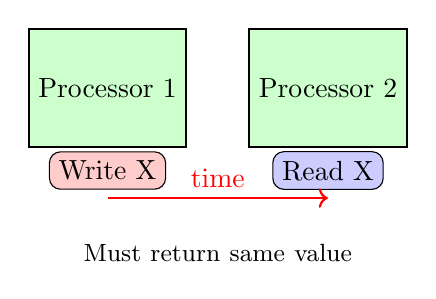
\begin{tikzpicture}[scale=0.7]
      % Scenario 1
      \node[draw, thick, fill=green!20, minimum width=2cm, minimum height=1.5cm] (p1) at (0,0) {Processor 1};
      \node[draw, thick, fill=green!20, minimum width=2cm, minimum height=1.5cm] (p2) at (4,0) {Processor 2};
      
      \node[draw, fill=red!20, rounded corners] at (0,-1.5) {Write X};
      \node[draw, fill=blue!20, rounded corners] at (4,-1.5) {Read X};
      
      \draw[->, thick, red] (0,-2) -- node[above] {time} (4,-2);
      
      \node[text width=4cm, align=center] at (2,-3) {\small Must return same value};
    \end{tikzpicture}
  \end{center}
\end{frame}

% Frame 4: MESI Protocol
\begin{frame}{MESI Protocol}
\begin{columns}[T]
\begin{column}{0.55\textwidth}
  \textbf{Each cache line can be in one of 4 states:}

  \vspace{0.3cm}

  \begin{tikzpicture}[every node/.style={font=\normalsize}]
    \node[draw, thick, fill=invalidcolor, minimum width=6.5cm, minimum height=0.9cm, align=left] (invalid) at (0,0) {
      \mesistate{I}{invalidcolor} \textbf{Invalid} -- Data is not valid
    };

    \node[draw, thick, fill=sharedcolor, minimum width=6.5cm, minimum height=0.9cm, align=left] (shared) at (0,-1.1) {
      \mesistate{S}{sharedcolor} \textbf{Shared} -- Valid, clean, may have copies
    };

    \node[draw, thick, fill=exclusivecolor, minimum width=6.5cm, minimum height=0.9cm, align=left] (exclusive) at (0,-2.2) {
      \mesistate{E}{exclusivecolor} \textbf{Exclusive} -- Valid, clean, no copies
    };

    \node[draw, thick, fill=modifiedcolor, minimum width=6.5cm, minimum height=0.9cm, align=left] (modified) at (0,-3.3) {
      \mesistate{M}{modifiedcolor} \textbf{Modified} -- Valid, dirty, no copies
    };
  \end{tikzpicture}
\end{column}

\begin{column}{0.45\textwidth}
  \centering
  \textbf{State Properties:}
  \vspace{0.2cm}

  \begin{tikzpicture}[
    cell/.style={minimum width=1.3cm, minimum height=0.6cm, align=center, font=\small},
    headercell/.style={cell, fill=gray!30, font=\small\bfseries},
  ]
    \matrix[matrix of nodes,
      column sep=0pt, row sep=0pt,
      ampersand replacement=\&,
      nodes={cell, draw=gray},
      column 1/.style={nodes={headercell, minimum width=1.5cm}},
      row 1/.style={nodes={headercell}},
    ] (m) {
      State \& Valid \& Dirty \& Copies? \\
      |[fill=invalidcolor]| I \& No \& -- \& maybe \\
      |[fill=sharedcolor]| S \& Yes \& No \& maybe \\
      |[fill=exclusivecolor]| E \& Yes \& No \& No \\
      |[fill=modifiedcolor]| M \& Yes \& Yes \& No \\
    };
  \end{tikzpicture}

  \vspace{0.4cm}
  \small
  \textbf{Key insight:}\\
  To modify data, must first obtain \textcolor{red}{\textbf{ownership}} (transition to M or E state)
\end{column}
\end{columns}
\end{frame}

% Macro for the multi-processor example frames
\newcommand{\mpexample}[8]{% {p1-cache}{p1-state}{p2-cache}{p2-state}{l2-content}{l2-bits}{memory}{description}
  \centering
  \begin{tikzpicture}[scale=0.7, every node/.style={font=\scriptsize}]
    % L2 Cache - split into two lines
    \node[draw, thick, fill=brown!20, minimum width=4.5cm, minimum height=1cm, align=center] (l2) at (1.5,-2.5) {L2 cache (shared)\\[2pt]#5};
 
    % Processor 1 - direct code instead of macro
    \node[draw, thick, fill=green!20, minimum width=2.2cm, minimum height=1.8cm, align=center, anchor=south west] (p1) at ([yshift=20]l2.north west) {};
    \node[above] at (p1.north) {\textbf{Processor 1}};
    
    % Processor 2 - direct code instead of macro
    \node[draw, thick, fill=green!20, minimum width=2.2cm, minimum height=1.8cm, align=center, anchor=south east] (p2) at ([yshift=20]l2.north east) {};
    \node[above] at (p2.north) {\textbf{Processor 2}};
    
    % L1 Caches with content - split into two lines
    \node[draw, thick, fill=lightgray!20, minimum width=1.9cm, minimum height=0.9cm, align=center] (l1p1) at (p1.center) {L1 cache\\[2pt]#1};
    \node[draw, thick, fill=lightgray!20, minimum width=1.9cm, minimum height=0.9cm, align=center] (l1p2) at (p2.center) {L1 cache\\[2pt]#3};
    
    % State indicators - positioned outside the cache box at lower right corner
    \ifx&#2&\else
      \ifnum\pdfstrcmp{#2}{modifiedcolor}=0
        \node[circle, draw, thick, fill=orange!70, minimum size=0.4cm, font=\tiny\bfseries] at ($(l1p1.south east)+(0.1,-0.1)$) {M};
      \else\ifnum\pdfstrcmp{#2}{exclusivecolor}=0
        \node[circle, draw, thick, fill=yellow!70, minimum size=0.4cm, font=\tiny\bfseries] at ($(l1p1.south east)+(0.1,-0.1)$) {E};
      \else\ifnum\pdfstrcmp{#2}{sharedcolor}=0
        \node[circle, draw, thick, fill=cyan!70, minimum size=0.4cm, font=\tiny\bfseries] at ($(l1p1.south east)+(0.1,-0.1)$) {S};
      \else\ifnum\pdfstrcmp{#2}{invalidcolor}=0
        \node[circle, draw, thick, fill=red!40, minimum size=0.4cm, font=\tiny\bfseries] at ($(l1p1.south east)+(0.1,-0.1)$) {I};
      \fi\fi\fi\fi
    \fi
    \ifx&#4&\else
      \ifnum\pdfstrcmp{#4}{modifiedcolor}=0
        \node[circle, draw, thick, fill=orange!70, minimum size=0.4cm, font=\tiny\bfseries] at ($(l1p2.south east)+(0.1,-0.1)$) {M};
      \else\ifnum\pdfstrcmp{#4}{exclusivecolor}=0
        \node[circle, draw, thick, fill=yellow!70, minimum size=0.4cm, font=\tiny\bfseries] at ($(l1p2.south east)+(0.1,-0.1)$) {E};
      \else\ifnum\pdfstrcmp{#4}{sharedcolor}=0
        \node[circle, draw, thick, fill=cyan!70, minimum size=0.4cm, font=\tiny\bfseries] at ($(l1p2.south east)+(0.1,-0.1)$) {S};
      \else\ifnum\pdfstrcmp{#4}{invalidcolor}=0
        \node[circle, draw, thick, fill=red!40, minimum size=0.4cm, font=\tiny\bfseries] at ($(l1p2.south east)+(0.1,-0.1)$) {I};
      \fi\fi\fi\fi
    \fi
    
   
    % Core valid bits
    \node[draw, thick, minimum width=1cm, minimum height=0.6cm, align=center] at ($(l2.east)+(0.9,0)$) {\tiny P1 P2\\[-1pt]#6};
    
    % Memory - split into two lines
    \node[draw, thick, fill=blue!20, minimum width=3.8cm, minimum height=0.9cm, align=center, anchor=north] (mem) at ([yshift=-20]l2.south) {Memory\\[2pt]#7};
    
    % Arrows with straight lines using |- syntax
    \draw[<->, thick] (p1.south) -- (p1 |- l2.north);
    \draw[<->, thick] (p2.south) -- (p2 |- l2.north);
    \draw[<->, thick] (l2.south) -- (mem.north);
  \end{tikzpicture}
}

% Frames 5-12: Multi-processor Example
\begin{frame}{Multi-processor Example: Step 1}
  \textbf{P1 reads address 1000}

  \begin{columns}
    \column{0.50\textwidth}
    \begin{itemize}
      \item P1 has a cache miss
      \item Data loaded from memory to L2
      \item L2 forwards to P1's L1
      \item Line marked as \stateE{} Exclusive in P1
    \end{itemize}

    \column{0.50\textwidth}
    \mpexample{[1000]: 5}{exclusivecolor}{}{}{[1000]: 5}{10}{[1000]: 5}{}
  \end{columns}
\end{frame}

\begin{frame}{Multi-processor Example: Step 2}
  \textbf{P1 writes address 1000}

  \begin{columns}
    \column{0.50\textwidth}
    \begin{itemize}
      \item P1 modifies the value: 5 → 6
      \item \stateE{} → \stateM{} (Modified)
      \item L2 still has old value (5)
      \item Memory still has old value (5)
    \end{itemize}

    \column{0.50\textwidth}
    \centering
    \mpexample{[1000]: 6}{modifiedcolor}{}{}{[1000]: 5}{10}{[1000]: 5}{}
  \end{columns}
\end{frame}

\begin{frame}{Multi-processor Example: Step 3}
  \textbf{P2 reads address 1000}

  \begin{columns}
    \column{0.50\textwidth}
    \begin{itemize}
      \item P2 has a cache miss
      \item L2 snoops address 1000 from P1
      \item P1 writes back modified data (6) to L2
      \item P1: \stateM{} → \stateS{}, P2: \stateI{} → \stateS{}
      \item L2 updated with new value (6)
    \end{itemize}

    \column{0.50\textwidth}
    \mpexample{[1000]: 6}{sharedcolor}{[1000]: 6}{sharedcolor}{[1000]: 6}{11}{[1000]: 5}{}
  \end{columns}
\end{frame}

\begin{frame}{Multi-processor Example: Step 4}
  \textbf{P2 requests ownership (RFO) for address 1000}

  \begin{columns}
    \column{0.50\textwidth}
    \begin{itemize}
      \item P2 wants to write to address 1000
      \item L2 sends snoop invalidate to P1
      \item P1: \stateS{} → \stateI{} (invalidated)
      \item P2: \stateS{} → \stateE{} (granted ownership)
      \item CVB updated: P1=0, P2=1
    \end{itemize}

    \column{0.50\textwidth}
    \mpexample{[1000]: 6}{invalidcolor}{[1000]: 6}{exclusivecolor}{[1000]: 6}{01}{[1000]: 5}{}
  \end{columns}
\end{frame}

\begin{frame}{Multi-processor Example: Step 5}
  \textbf{P2 writes address 1000}
  \begin{columns}
    \column{0.50\textwidth}
    \begin{itemize}
      \item P2 modifies the value: 6 → 7
      \item P2: \stateE{} → \stateM{} (local write)
      \item P1 remains \stateI{}
      \item L2 and Memory still have old values
    \end{itemize}

    \column{0.50\textwidth}
    \mpexample{[1000]: 6}{invalidcolor}{[1000]: 7}{modifiedcolor}{[1000]: 6}{01}{[1000]: 5}{}
  \end{columns}
\end{frame}

\begin{frame}{Multi-processor Example: Step 6}
  \textbf{L2 evicts address 1000}

  \begin{columns}
    \column{0.50\textwidth}
    \begin{itemize}
      \item L2 needs to evict line 1000 (capacity)
      \item L2 sends snoop invalidate to P2
      \item P2 responds with modified data (7)
      \item L2 writes back to memory: 5 → 7
      \item All caches now \stateI{}
    \end{itemize}

    \column{0.50\textwidth}
    \mpexample{--}{invalidcolor}{--}{invalidcolor}{(evicted)}{00}{[1000]: 7}{}
  \end{columns}
\end{frame}

% Summary frame
\begin{frame}{Cache Coherence Summary}
  \begin{columns}
    \column{0.5\textwidth}
    \textbf{Key Concepts:}
    \begin{itemize}
      \item L2 cache reduces L1 miss penalty
      \item Inclusive L2 simplifies coherence
      \item MESI protocol maintains consistency
      \item Snooping enables cache coherence
    \end{itemize}
    
    \vspace{0.5cm}
    
    \textbf{Performance Implications:}
    \begin{itemize}
      \item Shared data causes invalidations
      \item False sharing can hurt performance
      \item Write-back reduces memory traffic
    \end{itemize}
    
    \column{0.5\textwidth}
    \begin{tikzpicture}[scale=0.8, every node/.style={font=\small}]
      % MESI state diagram
      \node[circle, draw, thick, fill=invalidcolor, minimum size=1.2cm] (I) at (0,0) {I};
      \node[circle, draw, thick, fill=sharedcolor, minimum size=1.2cm] (S) at (3,0) {S};
      \node[circle, draw, thick, fill=exclusivecolor, minimum size=1.2cm] (E) at (0,-3) {E};
      \node[circle, draw, thick, fill=modifiedcolor, minimum size=1.2cm] (M) at (3,-3) {M};
      
      % Transitions (simplified)
      \draw[->, thick] (I) -- node[above] {\tiny Read} (E);
      \draw[->, thick] (I) -- node[above] {\tiny Read} (S);
      \draw[->, thick] (E) -- node[right] {\tiny Write} (M);
      \draw[->, thick] (S) -- node[below] {\tiny Write} (M);
      \draw[->, thick, bend left=20] (M) -- node[right] {\tiny Snoop} (S);
      \draw[->, thick, bend left=20] (E) -- node[left] {\tiny Snoop} (S);
      
      \node[below] at (1.5,-4) {\textbf{MESI State Transitions}};
    \end{tikzpicture}
  \end{columns}
\end{frame}





\begin{frame}{Multi-processor System: Inclusion}
  \begin{itemize}
    \item \textbf{L2 needs to keep track of the presence of each line in each of the processors}
    \begin{itemize}
      \item Determine if it needs to send a snoop to a processor
      \item Determine in what state to provide a requested line (S,E)
      \item[$\Rightarrow$] Need to guarantee that the L1 caches in each processor are inclusive of the L2 cache
    \end{itemize}
    \vspace{0.2cm}
    \item \textbf{When L2 evicts a line}
    \begin{itemize}
      \item L2 sends a snoop invalidate to all processors that have it
      \item If the line is modified in the L1 cache of one of the processors (in which case it exist only in that processor)
      \begin{itemize}
        \item The processor responds by sending the updated value to L2
        \item When the line is evicted from L2, the updated value gets written to memory
      \end{itemize}
    \end{itemize}
  \end{itemize}
\end{frame}

\begin{frame}{Global Observation (GO)}
\begin{itemize}
  \item A write is \textbf{globally observed} when any subsequent read by any processor returns its value
  \item Data for an RFO can be sent early, but GO cannot be granted until invalidations complete
  \item Prevents ordering violations where other cores still use stale values
\end{itemize}
\end{frame}

\begin{frame}{Inclusion vs. Non-Inclusive Designs}
\begin{itemize}
  \item Inclusive L2 is simple but wastes space when L2 is not much larger than L1
  \item \textbf{Non-inclusive} design: a separate \textbf{snoop filter} (tags + per-core valid bits) tracks sharers
  \item L1 and L2 can be mutually exclusive; L2 acts as a victim cache for L1
\end{itemize}
\end{frame}

\begin{frame}{Cache Optimization Summary}
\begin{center}
\footnotesize
\begin{tabular}{lccc}
\toprule
\textbf{Technique} & \textbf{Miss Rate} & \textbf{Miss Penalty} & \textbf{Hit Time}\\
\midrule
\textbf{Miss Rate Reduction:} & & & \\
\quad Larger Block Size & + & -- & \\
\quad Higher Associativity & + & & -- \\
\quad Victim Caches & + & & \\
\quad Pseudo-Associative Caches & + & & \\
\quad HW Prefetching of Instr/Data & + & & \\
\quad Compiler Controlled Prefetching & + & & \\
\quad Compiler Reduce Misses & + & & \\
\midrule
\textbf{Miss Penalty Reduction:} & & & \\
\quad Priority to Read Misses & & + & \\
\quad Sub-block Placement & & + & + \\
\quad Early Restart \& Critical Word 1st & & + & \\
\quad Non-Blocking Caches & & + & \\
\quad Second Level Caches & & + & \\
\bottomrule
\end{tabular}
\end{center}
\end{frame}

\begin{frame}{Memory Models}
\begin{itemize}
  \item \textbf{What is a memory model?}
  \begin{itemize}
    \item Defines the ordering guarantees and visibility of memory operations
    \item Specifies which memory operation reorderings are allowed by the architecture
    \item Contract between hardware and software
  \end{itemize}

  \vspace{0.3cm}

  \item \textbf{Why do we need memory models?}
  \begin{itemize}
    \item Modern processors reorder instructions for performance (out-of-order execution)
    \item Caches and write buffers affect when stores become visible to other processors
    \item Without a clear model, multi-threaded programs would be impossible to reason about
  \end{itemize}

  \vspace{0.3cm}

  \item \textbf{Memory model spectrum}
  \begin{itemize}
    \item \textbf{Sequential Consistency (SC)}: All operations appear in program order (strongest, slowest)
    \item \textbf{Total Store Order (TSO)}: x86 model — allows some reordering for performance
    \item \textbf{Relaxed Models}: ARM, RISC-V — allow more reordering (weakest, fastest)
  \end{itemize}
\end{itemize}
\end{frame}

\begin{frame}{The Happens-Before Relation}
\begin{itemize}
  \item \textbf{Happens-before ($\rightarrow$) is a partial order on memory operations}
  \begin{itemize}
    \item If operation $A$ happens-before operation $B$ (written $A \rightarrow B$), then:
    \begin{itemize}
      \item The effects of $A$ are visible to $B$
      \item $A$ cannot be reordered after $B$
    \end{itemize}
  \end{itemize}

  \vspace{0.3cm}

  \item \textbf{Sources of happens-before relations}
  \begin{itemize}
    \item \textbf{Program order}: Within a single thread, if instruction $I_1$ comes before $I_2$ in program order, and the memory model preserves that order, then $I_1 \rightarrow I_2$
    \item \textbf{Synchronization}: Acquiring a lock happens-before releasing it
    \item \textbf{Transitivity}: If $A \rightarrow B$ and $B \rightarrow C$, then $A \rightarrow C$
  \end{itemize}

  \vspace{0.3cm}

  \item \textbf{Key insight}
  \begin{itemize}
    \item Memory models specify which program-order pairs create happens-before
    \item If there's no happens-before relation, operations may be reordered
    \item Violations occur when observed behavior contradicts happens-before
  \end{itemize}
\end{itemize}
\end{frame}

\begin{frame}{x86 Memory Ordering: Rules}
\begin{enumerate}
  \item Loads are not reordered with other loads.
  \item Stores are not reordered with other stores.
  \item Stores are not reordered with older loads.
  \item Loads may reorder with older stores to \emph{different} locations, but not to the same location.
  \item Causality respected; stores to the same location have a total order.
  \item Locked instructions are totally ordered and not reordered with loads/stores.
\end{enumerate}
\end{frame}

\begin{frame}[fragile]{x86 Ordering: Loads and Stores Keep Their Own Order}
\begin{itemize}
  \item I.e., loads are seen in program order, and stores are seen in program order
\end{itemize}
Initial: \texttt{x=y=0}. The outcome \texttt{r1=1, r2=0} is \textbf{not} allowed.\\[2pt]
\begin{columns}[T]
\column{0.48\textwidth}
\textbf{Processor 0}
\begin{minted}[fontsize=\small]{text}
Store [X] <- 1   // S1
Store [Y] <- 1   // S2
\end{minted}
\column{0.48\textwidth}
\textbf{Processor 1}
\begin{minted}[fontsize=\small]{text}
r1 <- Load [Y]   // L1
r2 <- Load [X]   // L2
\end{minted}
\end{columns}

\vspace{0.2cm}
\textbf{Happens-before analysis:}
\begin{itemize}
  \item On P0: $\text{S1} \rightarrow \text{S2}$ (stores in program order)
  \item On P1: $\text{L1} \rightarrow \text{L2}$ (loads in program order)
  \item If L1 reads S2's value (r1=1), then S2 happened, so S1 must have happened too
  \item Since $\text{L1} \rightarrow \text{L2}$, L2 must see S1's effect $\Rightarrow$ r2=1
  \item Therefore r1=1, r2=0 violates happens-before
\end{itemize}
\end{frame}

\begin{frame}[fragile]{x86 Ordering: Stores Not Reordered with Older Loads}
Initial: \texttt{x=y=0}. The outcome \texttt{r1=1, r2=1} is \textbf{not} allowed.\\[2pt]
\begin{columns}[T]
\column{0.48\textwidth}
\textbf{Processor 0}
\begin{minted}[fontsize=\small]{text}
r1 <- Load [X]   // L1
Store [Y] <- 1   // S1
\end{minted}
\column{0.48\textwidth}
\textbf{Processor 1}
\begin{minted}[fontsize=\small]{text}
r2 <- Load [Y]   // L2
Store [X] <- 1   // S2
\end{minted}
\end{columns}

\vspace{0.2cm}
\textbf{Happens-before analysis:}
\begin{itemize}
  \item On P0: $\text{L1} \rightarrow \text{S1}$ (store not reordered before load)
  \item On P1: $\text{L2} \rightarrow \text{S2}$ (store not reordered before load)
  \item If r1=1, then L1 observed S2, meaning S2 happened
  \item Since $\text{L2} \rightarrow \text{S2}$, L2 happened before S2
  \item Since $\text{L1} \rightarrow \text{S1}$, S1 happens after L1 observed S2
  \item Therefore, L2 should observe S1 (r2=1 or see S1 happen later)
  \item But if both r1=1 and r2=1, there's a cycle: impossible!
\end{itemize}
\end{frame}

\begin{frame}[fragile]{x86 Ordering: Loads May Reorder with Older Stores to Different Locations}
Initial: \texttt{x=y=0}. Outcome \texttt{r1=0, r2=0} is \textbf{allowed}.\\[2pt]
\begin{columns}[T]
\column{0.48\textwidth}
\textbf{Processor 0}
\begin{minted}[fontsize=\small]{text}
Store [X] <- 1   // S1
r1 <- Load [Y]   // L1
\end{minted}
\column{0.48\textwidth}
\textbf{Processor 1}
\begin{minted}[fontsize=\small]{text}
Store [Y] <- 1   // S2
r2 <- Load [X]   // L2
\end{minted}
\end{columns}

\vspace{0.2cm}
\textbf{Happens-before analysis:}
\begin{itemize}
  \item On P0: S1 and L1 access \emph{different} locations $\Rightarrow$ \textbf{no} happens-before!
  \item On P1: S2 and L2 access \emph{different} locations $\Rightarrow$ \textbf{no} happens-before!
  \item Without happens-before, loads can execute before stores
  \item Possible execution: L1 and L2 both execute first (see 0), then S1 and S2
  \item This outcome (r1=0, r2=0) is allowed because no happens-before is violated
\end{itemize}
\end{frame}

\begin{frame}[fragile]{x86 Ordering: Causality and Transitive Visibility}
Initial: \texttt{x=y=0}. Outcome \texttt{r1=1, r2=1, r3=0} is \textbf{not} allowed.\\[2pt]
\begin{columns}[T]
\column{0.32\textwidth}
{\footnotesize\textbf{Processor 0}}
\begin{minted}[fontsize=\scriptsize]{text}
Store [X] <- 1   // S1
\end{minted}
\column{0.32\textwidth}
{\footnotesize\textbf{Processor 1}}
\begin{minted}[fontsize=\scriptsize]{text}
r1 <- Load [X]   // L1
Store [Y] <- 1   // S2
r2 <- Load [Y]   // L2
\end{minted}
\column{0.32\textwidth}
{\footnotesize\textbf{Processor 2}}
\begin{minted}[fontsize=\scriptsize]{text}
r3 <- Load [X]   // L3
\end{minted}
\end{columns}

\vspace{0.1cm}
{\small
\textbf{Happens-before analysis (transitivity):}
\begin{itemize}
  \item If r1=1: L1 observed S1 $\Rightarrow$ $\text{S1} \rightarrow \text{L1}$
  \item On P1: $\text{L1} \rightarrow \text{S2} \rightarrow \text{L2}$ (program order)
  \item If r2=1: L2 observed S2 $\Rightarrow$ $\text{S2} \rightarrow \text{L2}$
  \item By transitivity: $\text{S1} \rightarrow \text{L1} \rightarrow \text{S2} \rightarrow \text{L2}$
  \item Since L2 observed S2, and S2 happened after S1, any subsequent load must see S1
  \item Therefore L3 must see S1 $\Rightarrow$ r3=1 (r3=0 violates transitivity)
\end{itemize}
}
\end{frame}

\end{document}